Automatic memory management or garbage collection greatly simplifies
development of large systems. However, garbage collection is usually
not used in real-time systems due to the unpredictable temporal
behavior of current implementations of a garbage collector. In this
chapter we describe a concurrent collector that is scheduled
periodically in the same way as ordinary application threads. We
provide an upper bound for the collector period so that the
application threads will never run out of memory. This chapter is
based on following papers:
\cite{jop:rtgc_sched,jop:scjgc,jop:nbobjcopy:jtres2008}.


\section{Introduction}

Garbage Collection (GC) is an essential part of the Java runtime
system. GC enables automatic dynamic memory management which is
essential to build large applications. Automatic memory management
frees the programmer from complex and error prone explicit memory
management (\code{malloc} and \code{free}).

However, garbage collection is considered unsuitable for real-time
systems due to the unpredictable blocking times introduced by the GC
work. One solution, used in the Real-Time Specification for Java
(RTSJ) \cite{rtsj}, introduces new thread types with program-managed,
scoped memory for dynamic memory requirements. This scoped memory
(and static memory called \emph{immortal} memory) is not managed by
the GC, and strict assignment rules between different memory areas
have to be checked at runtime. This programming model differs largely
from standard Java and is difficult to use \cite{Niessner03,
conf/isorc/PizloFHV04}.

We believe that for the acceptance of Java for real-time systems, the
restrictions imposed by the RTSJ are too strong. To simplify creation
of possible large real-time applications, most of the code should be
able to use the GC managed heap. For a collector to be used in
real-time systems two points are essential:
\begin{itemize}
    \item The GC has to be incremental with a short maximum blocking time
    that has to be known
    \item The GC has to keep up with the garbage generated by the
    application threads to avoid out-of-memory stalls
\end{itemize}
The first point is necessary to limit interference between the GC
thread and high-priority threads. It is also essential to minimize
the overhead introduced by read- and write-barriers, which are
necessary for synchronization between the GC thread and the
application threads. The design of a GC within these constraints is
the topic of this chapter.

The second issue that has to be considered is scheduling the GC so
that the GC collects enough garbage. The memory demands (static and
dynamic) by the application threads have to be analyzed. These
requirements, together with the properties of the GC, result in
scheduling parameters for the GC thread. We will provide a solution
to calculate the maximum period of the GC thread that will collect
enough memory in each collector cycle so we will never run out of
memory. The collector cycle depends on the heap size and the
allocation rate of the application threads.

To distinguish between other garbage collectors and a collector for
(hard) real-time systems we define a real-time collector as follows:

\begin{quote}
    A real-time garbage collector provides time predictable
    automatic memory management for tasks with a bounded memory
    allocation rate with minimal temporal interference to tasks
    that use only static memory.
\end{quote}


The collector presented in this chapter is based on the work by
Steele \cite{gc:steele75},  Dijkstra \cite{gc:dijkstra78} and Baker
\cite{gc:baker78}. However, the copying collector is changed to
perform the copy of an object concurrently by the collector and not
as part of the mutator work. Therefore we name it
\emph{concurrent-copy} collector.

We will use the terms first introduced by Dijkstra with his
\emph{On-the-Fly} concurrent collector \cite{gc:dijkstra78}. The
application is called the \emph{mutator} to reinforce that the
application changes (mutates) the object graph while the GC does the
collection work. The GC process is simply called \emph{collector}. In
the following discussion we will use the color scheme of white, gray,
and black objects:

\begin{description}
    \item[Black] indicates that the object and all immediate
    descendants have been visited by the collector.
    \item[Grey] objects have been visited, but the descendants may
    not have been visited by the collector, or the mutator has
    changed the object.
    \item[White] objects are unvisited. At the beginning of a GC
        cycle all objects are white. At the end of the tracing,
        all white objects are garbage.
\end{description}

At the end of a collection cycle all black objects are live (or
floating garbage) and all white objects are garbage.

\subsection{Incremental Collection}

An incremental collector can be realized in two ways: either by doing
part of the work on each allocation of a new object or by running the
collector as an independent process. For a single-threaded
application, the first method is simpler as less synchronization
between the application and the collector is necessary. For a
multi-threaded environment there is no advantage by interleaving
collector work with object allocation. In this case we need
synchronization between the collector work done by one thread and the
manipulation of the object graph performed by the other mutator
thread. Therefore we will consider a concurrent solution where the
collector runs in its own thread or processor. It is even possible to
realize the collector as dedicated hardware \cite{gc:flavius}.

\subsection{Conservatism}

Incremental collector algorithms are conservative, meaning that
objects becoming unreachable during collection are not collected by
the collector --- they are floating garbage. Many approaches exist to
reduce this conservatism in the general case. However, algorithms
that completely avoid floating garbage are impractical. For different
conservative collectors the worst-case bounds are all the same (i.e.,
all objects that become unreachable during collection remain floating
garbage). Therefore the level of conservatism is not an issue for
real-time collectors.

\subsection{Safety Critical Java}

In \cite{jop:scjava} a profile for safety critical Java (SCJ) is
defined. SCJ has two interesting properties that may simplify the
implementation of a real-time collector. Firstly, the split between
initialization and mission phase, and secondly the simplified
threading model (which also mandates that self-blocking operations
are illegal in the mission phase).  During initialization of the
application a SCJ virtual machine does not have to meet any real-time
constraints (other than possibly a worst case bound on the entire
initialization phase). It is perfectly acceptable to use a
non-real-time GC implementation during this phase -- even a
stop-the-world GC. As the change from initialization to mission phase
is explicit, it is clear when the virtual machine must initiate
real-time collection and which code runs during the mission phase.


Simplifying the threading model has the following advantage, if the
collector thread runs at a lower priority than all other threads in
the system, it is the case that when it runs \emph{all} other threads
have returned from their calls to \code{run()}. This is trivially
true due to the priority preemptive scheduling
discipline.\footnote{If we would allow blocking in the application
threads, we would also need to block the GC thread.} Any thread that
has not returned from its \code{run()} method will preempt the GC
until it returns. This has the side effect that the GC will never see
a root in the call stack of another thread. Therefore, the usually
atomic operation of scanning call stacks can be omitted in the
mission phase. We will elaborate on this property in
Section~\ref{sec:scj:simple}.


\section{Scheduling of the Collector Thread}
\label{sec:gcsched}

The collector work can be scheduled either \emph{work} based or
\emph{time} based. On a work based scheduling, as performed in
\cite{gc:siebert:phd}, an incremental part of the collector work is
performed at object allocation. This approach sounds quite natural as
threads that allocate more objects have to pay for the collector
work. Furthermore, no additional collector thread is necessary. The
main issue with this approach is to determine how much work has to be
done on each allocation -- a non trivial question as collection work
consists of different phases. A more subtle question is: Why should a
high frequency (and high priority) thread increase its WCET by
performing collector work that does not have to be done at that
period? Leaving the collector work to a thread with a longer period
allows higher utilization of the system.

On a time based scheduling of the collector work, the collector runs
in its own thread. Scheduling this thread as a \emph{normal}
real-time thread is quite natural for a hard real-time system. The
question is: which priority to assign to the collector thread? The
Metronome collector \cite{gc:bacon03} uses the highest priority for
the collector. Robertz and Henriksson \cite{780745} and Schoeberl
\cite{jop:rtgc_sched} argue for the lowest priority. When building
hard real-time systems the answer must take scheduling theory into
consideration: the priority is assigned according to the period,
either rate monotonic \cite{321743} or more general deadline
monotonic \cite{Audsley-etal91}. Assuming that the period of the
collector is the longest in the system and the deadline equals the
period the collector gets the lowest priority.

In this section we provide an upper bound for the collector period
so that the application threads will never run out of memory. The
collector period, besides the WCET of the collector, is the single
parameter of the collector that can be incorporated in standard
schedulability analysis.

The following symbols are used in this section: heap size for a
mark-compact collector ($H_{MC}$) and for a concurrent-copying
collector ($H_{CC}$) containing both semi-spaces, period of the GC
thread ($T_{GC}$), period of a single mutator thread ($T_M$), period
of mutator thread $i$ ($T_i$) from a set of threads, and memory
amount allocated by a single mutator ($a$) or by mutator $i$ ($a_i$)
from a set of threads.

We assume that the mutator allocates all memory at the start of the
period and the memory becomes garbage at the end. In other words the
memory is live for one period. This is the worst-case,\footnote{See
Section~\ref{sec:wc:live} for an example where the worst-case
lifetime is two periods.} but very common as we can see in the
following code fragment.
\begin{samepage}
\begin{lstlisting}
    for (;;) {
        Node n = new Node();
        work(n);
        waitForNextPeriod();
    }
\end{lstlisting}
\end{samepage}
The object \code{Node} is allocated at the start of the period and
\code{n} will reference it until the next period when a new
\code{Node} is created and assigned to \code{n}. In this example we
assume that no reference to \code{Node} is stored (inside
\code{work}) to an object with a longer lifetime.


\subsection{An Example} \label{sec:example}

\begin{figure}
\begin{center}
    \input{jvm/exmc.latex}
    \caption{Heap usage during a mark-compact collection cycle}
\label{fig:exmc}
\end{center}
\end{figure}

\begin{figure}
\begin{center}
    \input{jvm/excc2.latex}
    \caption{Heap usage during a concurrent-copy collection cycle}
\label{fig:excc}
\end{center}
\end{figure}


We start our discussion with a simple example\footnote{The relation
between the heap size and the mutator/collector proportion is an
arbitrary value in this example. We will provide the exact values in
the next sections.} where the collector period is 3 times the mutator
period ($T_{GC} = 3 T_M$) and a heap size of 8 objects ($8a$). We
show the heap during one GC cycle for a mark-compact and a
concurrent-copy collector. The following letters are used to show the
status of a memory cell (that contains one object from the mutator in
this example) in the heap: $g_i$ is garbage from mutator cycle $i$,
$l$ is the live memory, and $f$ is floating garbage. We assume that
all objects that become unreachable during the collection remain
floating garbage.

Figure~\ref{fig:exmc} shows the changes in the heap during one
collection cycle. At the start there are three objects ($g_1$,
$g_2$, and $g_3$) left over from the last cycle (floating garbage)
which are collected by the current cycle and one live object $l_4$.
During the collection the live objects become unreachable and are
now floating garbage (e.g. $f_4$ in the second sub-figure). At the
end of the cycle, just before compacting, we have three garbage
cells ($g_1$-$g_3$), three floating garbage cells ($f_4$-$f_6$) and
one live cell $l_7$. Compaction moves the floating garbage and the
live cell to the start of the heap and we end up with four free
cells. The floating garbage will become garbage in the next
collection cycle and we start over with the first sub-figure with
three garbage cells and one live cell.

Figure~\ref{fig:excc} shows one collection cycle of the
concurrent-copy collector. We have two memory spaces: the
\emph{from-space} and the \emph{to-space}. Again we start the
collection cycle with one live cell and three garbage cells left over
from the last cycle. Note that the order of the cells is different
from the previous example. New cells are allocated in the to-space
from the top of the heap, whereas moved cells are allocated from the
bottom of the heap. The second sub-figure shows a snapshot of the
heap during the collection: formerly live object $l_4$ is already
floating garbage $f_4$ and copied into to-space. A new cell $l_5$ is
allocated in the to-space. Before the flip of the two semi-spaces the
from-space contains the three garbage cells ($g_1$-$g_3$) and the
to-space the three floating garbage cells ($f_4$-$f_6$) and one live
cell $l_7$. The last sub-figure shows the heap after the flip: The
from-space contains the three floating cells which will be garbage
cells in the next cycle and the one live cell. The to-space is now
empty.

From this example we see that the necessary heap size for a
mark-compact collector is similar to the heap size for a copying
collector. We also see that the compacting collector has to move
more cells (all floating garbage cells and the live cell) than the
copying collector (just the one cell that is live at the beginning
of the collection).


\subsection{Minimum Heap Size} \label{sec:min:heap}

In this section we show the memory bounds for a mark-compact
collector with a single heap memory and a concurrent-copying
collector with the two spaces \emph{from-space} and \emph{to-space}.

\subsubsection{Mark-Compact} \label{sec:gcsched:mc}

For the mark-compact collector, the heap $H_{MC}$ can be divided into
allocated memory $M$ and free memory $F$
%
\begin{equation}\label{equ:mcheap}
    H_{MC} = M + F = G + \overline{G} + L + F
\end{equation}
%
where $G$ is garbage at the start of the collector cycle that will
be reclaimed by the collector. Objects that become unreachable
during the collection cycle and will not be reclaimed are floating
garbage $\overline{G}$. These objects will be detected in the next
collection cycle. We assume the worst case that all objects that die
during the collection cycle will not be detected and therefore are
floating garbage. $L$ denotes all live,i.e.\  reachable, objects.
$F$ is the remaining free space.

We have to show that we will never run out of memory during a
collection cycle ($F\ge0$). The amount of allocated memory $M$ has to
be less than or equal to the heap size $H_{MC}$

\begin{equation}\label{equ:mcheapmin}
    H_{MC} \ge M = G + \overline{G} + L
\end{equation}


In the following proof the superscript $n$ denotes the collection
cycle. The subscript letters $S$ and $E$ denote the value at the
start and the end of the cycle, respectively.

\begin{lemma}

For a collection cycle the amount of allocated memory $M$ is bounded
by the maximum live data $L_{max}$ at the start of the collection
cycle and two times $A_{max}$, the maximum data allocated by the
mutator during the collection cycle.

\begin{equation}\label{equ:mc:lemma}
    M \le L_{max} + 2 A_{max}
\end{equation}

\end{lemma}

\begin{proof}

During a collection cycle $G$ remains constant. All live data that
becomes unreachable will be floating garbage. Floating garbage
$\overline{G}_E$ at the end of cycle $n$ will be detected (as
garbage $G$) in cycle $n+1$.
%
\begin{equation}\label{equ:flg}
    G^{n+1} = \overline{G}_E^n
\end{equation}
%
The mutator allocates $A$ memory and transforms part of this memory
and part of the live data at the start $L_S$ to floating garbage
$\overline{G}_E$ at the end of the cycle. $L_E$ is the data that is
still reachable at the end of the cycle.
%
\begin{equation}\label{equ:trans}
    L_S + A = L_E + \overline{G}_E
\end{equation}
%
with $A \le A_{max}$ and $L_S \le L_{max}$. A new collection-cycle
start immediately follows the end of the former cycle. Therefore the
live data remains unchanged.
%
\begin{equation}\label{equ:ldata}
    L_S^{n+1} = L_E^{n}
\end{equation}

We will show that (\ref{equ:mc:lemma}) is true for cycle 1. At the
start of the first cycle we have no garbage ($G=0$) and no live data
($L_S=0$). The heap contains only free memory.
%
\begin{equation}\label{equ:mc:start}
    M_S^1 = 0
\end{equation}
%
During the collection cycle the mutator allocates $A^1$ memory. Part
of this memory will be live at the end and the remaining will be
floating garbage.
%
\begin{equation}\label{equ:mc:cyc1:A}
    A^1 = L_E^1 + \overline{G}_E^1
\end{equation}
%
Therefore at the end of the first cycle
%
\begin{align}
\nonumber
    M_E^1 & = L_E^1 + \overline{G}_E^1\\
    M^1   & = A^1
\end{align}
%
As $A^1 \le A_{max}$ (\ref{equ:mc:lemma}) is fulfilled for cycle 1.

Under the assumption that (\ref{equ:mc:lemma}) is true for cycle
$n$, we have to show that (\ref{equ:mc:lemma}) holds for cycle
$n+1$.

\begin{equation}
    M^{n+1} \le L_{max} + 2 A_{max}
\end{equation}

\begin{align}
    M^n & = G^n + \overline{G}_E^n + L_E^n\\
    M^{n+1} & = G^{n+1} + \overline{G}_E^{n+1} + L_E^{n+1}\\
\nonumber
            & = \overline{G}_E^n + L_S^{n+1} + A^{n+1}
                & \mbox{apply (\ref{equ:flg}) and (\ref{equ:trans})}\\
\nonumber
            & = \overline{G}_E^n + L_E^{n} + A^{n+1}
                & \mbox{apply (\ref{equ:ldata})}\\
            & = L_S^{n} + A^n + A^{n+1}
                & \mbox{apply (\ref{equ:trans})}
\end{align}

As $L_S \le L_{max}$, $A^n \le A_{max}$ and $A^{n+1} \le A_{max}$

\begin{equation}
    M^{n+1} \le L_{max} + 2 A_{max}
\end{equation}


\end{proof}

\subsubsection{Concurrent-Copy}

In the following section we will show the memory bounds for a
concurrent-copying collector with the two spaces \emph{from-space}
and \emph{to-space}. We will use the same symbols as in
Section~\ref{sec:gcsched:mc} and denote the maximum allocated memory
in the from-space as $M_{From}$ and the maximum allocated memory in
the to-space as $M_{To}$.

For a copying-collector the heap $H_{CC}$ is divided in two equal
sized spaces $H_{From}$ and $H_{To}$. The amount of allocated memory
$M$ in each semi-space has to be less than or equal to
$\frac{H_{CC}}{2}$
%
\begin{equation}\label{equ:ccheapmin}
    H_{CC} = H_{From} + H_{To} \ge 2M
\end{equation}
%

\begin{lemma}

For a collection cycle, the amount of allocated memory $M$ in each
semi-space is bounded by the maximum live data $L_{max}$ at the start
of the collection cycle and $A_{max}$, the maximum data allocated by
the mutator during the collection cycle.

\begin{equation}\label{equ:cc:lemma}
    M \le L_{max} + A_{max}
\end{equation}

\end{lemma}

\begin{proof}

Floating garbage at the end of cycle $n$ will be detectable garbage
in cycle $n+1$
%
\begin{equation}\label{equ:cc:flg}
    G^{n+1} = \overline{G}_E^n
\end{equation}
%
Live data at the end of cycle $n$ will be the live data at the start
of cycle $n+1$

\begin{equation}\label{equ:cc:ldata}
    L_S^{n+1} = L_E^{n}
\end{equation}


The allocated memory $M_{From}$ in the from-space contains garbage
$G$ and the live data at the start $L_s$.
%
\begin{equation}
    M_{From} = G + L_S
\end{equation}
%
All new objects are allocated in the to-space. Therefore the memory
requirement for the from-space does not change during the collection
cycle. All garbage $G$ remains in the from-space and the to-space
only contains floating garbage and live data.
%
\begin{equation}
    M_{To} = \overline{G} + L
\end{equation}
%
At the start of the collection cycle, the to-space is completely
empty.
%
\begin{equation}
    M_{To\_S} = 0
\end{equation}
%
During the collection cycle all live data is copied into the
to-space and new objects are allocated in the to-space.

\begin{equation}
    M_{To\_E} = L_S + A
\end{equation}

At the end of the collector cycle, the live data from the start $L_S$
and new allocated data $A$ stays either live at the end $L_E$ or
becomes floating garbage $\overline{G}_E$.

\begin{equation}
    L_S + A = L_E + \overline{G}_E
\end{equation}

For the first collection cycle there is no garbage ($G=0$) and no
live data at the start ($L_S=0$), i.e.\ the from-space is empty
($M_{From}^1=0$). The to-space will only contain all allocated data
$A^1$, with $A^1 \le A_{max}$, and therefore (\ref{equ:cc:lemma}) is
true for cycle 1.

Under the assumption that (\ref{equ:cc:lemma}) is true for cycle
$n$, we have to show that (\ref{equ:cc:lemma}) holds for cycle
$n+1$.

\begin{align}
\nonumber
    M_{From}^{n+1} & \le L_{max} + A_{max}\\
    M_{To}^{n+1}   & \le L_{max} + A_{max}
\end{align}



At the start of a collection cycle, the spaces are flipped and the
new to-space is cleared.
%
\begin{align}
\nonumber
    H_{From}^{n+1} & \Leftarrow H_{To}^n\\
    H_{To}^{n+1}   & \Leftarrow \emptyset
\end{align}
%
The from-space:
%
\begin{align}
    M_{From}^{n}  & = G^n + L_S^n\\
    M_{From}^{n+1} & = G^{n+1} + L_S^{n+1}\\
\nonumber
                   & = \overline{G}_E^n + L_E^n\\
                   & = L_S^n + A^n
\end{align}
%
As $L_S \le L_{max}$ and $A^n \le A_{max}$
%
\begin{equation}
    M_{From}^{n+1} \le L_{max} + A_{max}
\end{equation}
%
The to-space:
%
\begin{align}
    M_{To}^{n}     & = \overline{G}_E^n + L_E^n\\
    M_{To}^{n+1}   & = \overline{G}_E^{n+1} + L_E^{n+1}\\
\nonumber
                   & = L_S^{n+1} + A^{n+1}\\
                   & = L_E^{n} + A^{n+1}
\end{align}
%
% end
%
As $L_E \le L_{max}$ and $A^{n+1} \le A_{max}$
%
\begin{equation}
    M_{To}^{n+1} \le L_{max} + A_{max}
\end{equation}
%
\end{proof}

From this result we can see that the dynamic memory consumption for a
mark-compact collector is similar to a concurrent-copy collector.
This is contrary to the common belief that a copy collector needs the
double amount of memory.

We have seen that the double-memory argument against a copying
collector does not hold for an incremental real-time collector. We
need double the memory of the allocated data during a collection
cycle in either case. The advantage of the copying collector over a
compacting one is that newly allocated data are placed in the
to-space and does not need to be copied. The compacting collector
moves all newly created data (that is mostly floating garbage) at the
compaction phase.

\subsection{Garbage Collection Period}

GC work is inherently periodic. After finishing one round of
collection the GC starts over. The important question is which is
the \emph{maximum} period the GC can be run so that the application
will never run out of memory. Scheduling the GC at a shorter period
does not hurt but decreases utilization.

In the following, we derive the maximum collector period that
guarantees that we will not run out of memory. The maximum period
$T_{GC}$ of the collector depends on $L_{max}$ and $A_{max}$ for
which safe estimates are needed.

We assume that the mutator allocates all memory at the start of the
period and the memory becomes garbage at the end. In other words the
memory is live for one period. This is the worst case, but very
common.

%\subsubsection{Single Mutator Thread}
%
%First we give an upper bound for the collector cycle time for a
%single mutator thread.
%
%\begin{lemma}
%
%For a single mutator thread with period $T_M$ that allocates memory
%``$a$" each period, the maximum collector period $T_{GC}$ that
%guarantees that we will not run out of memory is
%
%\begin{align}\label{sth:mc:lemma}
%    T_{GC} & \le T_M\left\lfloor\frac{H_{MC}-a}{2a}\right\rfloor\\
%    \label{sth:cc:lemma}
%    T_{GC} & \le T_M\left\lfloor\frac{H_{CC}-2a}{2a}\right\rfloor
%\end{align}
%
%\end{lemma}
%
%\begin{proof}
%The maximum live data referenced by a single mutator is the maximum
%data allocated by the mutator in a single cycle.
%\begin{equation}
%    L_{max} = a
%\end{equation}
%A single mutator allocates $a$ memory during the period $T_M$.
%Therefore the maximum allocation during the collector period
%$T_{GC}$ is
%%
%\begin{equation}
%    A_{max} = a \left\lceil\frac{T_{GC}}{T_{M}}\right\rceil
%\end{equation}
%%
%Using equations (\ref{equ:mcheapmin}) and (\ref{equ:mc:lemma}) we
%get the minimum heap size $H_{MC}$ for a mark-compact collector
%%
%\begin{align}
%\nonumber
%    H_{MC} & \ge L_{max} + 2 A_{max}\\
%    H_{MC} & \ge a \left(1 + 2
%    \left\lceil\frac{T_{GC}}{T_{M}}\right\rceil\right)
%\end{align}
%%
%Equations (\ref{equ:ccheapmin}) and (\ref{equ:cc:lemma}) result in
%the minimum heap size $H_{CC}$, containing both semi-spaces, for the
%concurrent-copy collector
%%
%\begin{align}
%\nonumber
%    H_{CC} & \ge 2(L_{max} + A_{max})\\
%    H_{CC} & \ge 2a \left(1 +
%    \left\lceil\frac{T_{GC}}{T_{M}}\right\rceil\right)
%\end{align}
%%
%The ceiling function covers the worst-case schedule between the
%collector thread and the mutator thread. We are interested in the
%maximum collector period $T_{GC}$ with a given heap size $H_{MC}$ or
%$H_{CC}$
%%
%\begin{align}
%    \label{equ:mc:ceil}
%    \left\lceil\frac{T_{GC}}{T_{M}}\right\rceil &
%    \le \frac{H_{MC}-a}{2a}
%\end{align}
%%
%\begin{align}
%    \label{equ:cc:ceil}
%    \left\lceil\frac{T_{GC}}{T_{M}}\right\rceil &
%    \le \frac{H_{CC}-2a}{2a}
%\end{align}
%%
%The maximum quotient ($\frac{T_{GC}}{T_{M}}$) that fulfills
%(\ref{equ:mc:ceil}) or (\ref{equ:cc:ceil}) is an integer $n$. $n$ is
%the largest integer that is less than or equal the right side of
%(\ref{equ:mc:ceil}) or (\ref{equ:cc:ceil}). Therefore we get for the
%mark-compact collector
%%
%\begin{align}
%    \label{equ:mc:floor}
%    \frac{T_{GC}}{T_{M}} &
%    \le \left\lfloor\frac{H_{MC}-a}{2a}\right\rfloor
%\end{align}
%%
%\begin{equation}
%    \Rightarrow T_{GC} \le T_M \left\lfloor\frac{H_{MC}-a}{2a}\right\rfloor
%\end{equation}
%%
%and for the concurrent-copy collector
%%
%\begin{align}
%    \label{equ:cc:floor}
%    \frac{T_{GC}}{T_{M}} &
%    \le \left\lfloor\frac{H_{CC}-2a}{2a}\right\rfloor
%\end{align}
%%
%\begin{equation}
%    \Rightarrow T_{GC} \le T_M \left\lfloor\frac{H_{CC}-2a}{2a}\right\rfloor
%\end{equation}
%
%\end{proof}
%
%\subsubsection{Several Mutator Threads}

In this section the upper bound of the period for the collector
thread is given for $n$ independent mutator threads.

\begin{theorem}
\label{sch:theorem}

For ``$n$" mutator threads with period $T_i$ where each thread
allocates $a_i$ memory each period, the maximum collector period
$T_{GC}$ that guarantees that we will not run out of memory is

\begin{align}\label{nth:mc:theorem}
    T_{GC} & \le \frac{H_{MC}-3\sum_{i=1}^{n} a_i}{2\sum_{i=1}^{n} \frac{a_i}{Ti}}\\
    \label{nth:cc:theorem}
    T_{GC} & \le \frac{H_{CC}-4\sum_{i=1}^{n} a_i}{2\sum_{i=1}^{n}
    \frac{a_i}{Ti}}
\end{align}

\end{theorem}

\begin{proof}

For $n$ mutator threads with periods $T_i$ and allocations $a_i$
during each period the values for $L_{max}$ and $A_{max}$ are
%
\begin{align}\label{nth:lmax}
    L_{max} & = \sum_{i=1}^{n} a_i\\
    A_{max} & = \sum_{i=1}^{n}
    \left\lceil\frac{T_{GC}}{T_i}\right\rceil a_i
\end{align}
%
The ceiling function for $A_{max}$ covers the individual worst cases
for the thread schedule and cannot be solved analytically. Therefore
we use a conservative estimation $A^{'}_{max}$ instead of $A_{max}$.
%
\begin{equation}
    A^{'}_{max} = \sum_{i=1}^{n} \left(\frac{T_{GC}}{T_i}+1\right)
    a_i
    \ge \sum_{i=1}^{n} \left\lceil\frac{T_{GC}}{T_i}\right\rceil a_i
\end{equation}
%
From (\ref{equ:mcheapmin}) and (\ref{equ:mc:lemma}) we get the
minimum heap size for a mark-compact collector
\begin{align}
\nonumber
    \label{equ:mc:mthreads:exact}
    H_{MC} & \ge L_{max} + 2 A_{max}\\
           & \ge \sum_{i=1}^{n} a_i + 2 \sum_{i=1}^{n}
             \left\lceil\frac{T_{GC}}{T_i}\right\rceil a_i
\end{align}
%
For a given heap size $H_{MC}$ we get the conservative upper bound
of the maximum collector period $T_{GC}$
%
\footnote{It has to be noted that this is a conservative value for
the maximum collector period $T_{GC}$. The maximum value
$T_{GC_{max}}$ that fulfills (\ref{equ:mc:mthreads:exact}) is in the
interval
%
\begin{equation}
\nonumber
    \left(\frac{H_{MC} - 3\sum_{i=1}^{n} a_i} {2\sum_{i=1}^{n}
        \frac{a_i}{T_i}},
        \frac{H_{MC} - \sum_{i=1}^{n} a_i} {2\sum_{i=1}^{n}
        \frac{a_i}{T_i}}\right)
\end{equation}
%
and can be found by an iterative search.}
%
\begin{align}
\nonumber
        2 A^{'}_{max} & \le H_{MC}-L_{max}
\\
        2\sum_{i=1}^{n} \left(\frac{T_{GC}}{T_i}+1\right) a_i
        & \le H_{MC}-L_{max}
\\
        T_{GC}
        & \le \frac{H_{MC}-L_{max} - 2\sum_{i=1}^{n} a_i}
        {2\sum_{i=1}^{n} \frac{a_i}{T_i}}
\end{align}
%
\begin{equation}
    \Rightarrow T_{GC} \le \frac{H_{MC}-3\sum_{i=1}^{n} a_i}{2\sum_{i=1}^{n} \frac{a_i}{Ti}}
\end{equation}
%
Equations (\ref{equ:ccheapmin}) and (\ref{equ:cc:lemma}) result in
the minimum heap size $H_{CC}$, containing both semi-spaces, for the
concurrent-copy collector
\begin{align} \nonumber
    H_{CC} & \ge 2 L_{max} + 2 A_{max}\\
           & \ge 2\sum_{i=1}^{n} a_i + 2\sum_{i=1}^{n}
              \left\lceil\frac{T_{GC}}{T_i}\right\rceil a_i
\end{align}
%
For a given heap size $H_{CC}$ we get the conservative upper bound
of the maximum collector period $T_{GC}$
\begin{align}
\nonumber
        2 A^{'}_{max} & \le H_{CC} - 2L_{max}
\\
        2\sum_{i=1}^{n} \left(\frac{T_{GC}}{T_i}+1\right) a_i
        & \le H_{CC} - 2L_{max}
\\
        T_{GC}
        & \le \frac{H_{CC} - 2L_{max} - 2\sum_{i=1}^{n} a_i}
        {2\sum_{i=1}^{n} \frac{a_i}{T_i}}
\end{align}
%
\begin{equation}
    \Rightarrow T_{GC} \le \frac{H_{CC}-4\sum_{i=1}^{n} a_i}{2\sum_{i=1}^{n} \frac{a_i}{Ti}}
\end{equation}
\end{proof}

\subsubsection{Producer/Consumer Threads} \label{sec:prod:cons}

So far we have only considered threads that do not share objects for
communication. This execution model is even more restrictive than
the RTSJ scoped memories that can be shared between threads. In this
section we discuss how our GC scheduling can be extended to account
for threads that share objects.

Object sharing is usually done by a producer and a consumer thread.
I.e.,\ one thread allocates the objects and stores references to
those objects in a way that they can be accessed by the other
thread. This other thread, the consumer, is in charge to \emph{free}
those objects after use.

An example of this sharing is a device driver thread that
periodically collects data and puts them into a list for further
processing. The consumer thread, with a longer period, takes all
available data from the list at the start of the period, processes
the data, and removes them from the list. During the data processing,
new data can be added by the producer. Note that in this case the
list will probably never be completely empty. This typical case
cannot be implemented by an RTSJ shared scoped memory. There would be
no point in the execution where the shared memory will be empty and
can get recycled.

The question now is how much data will be alive in the worst case.
We denote $T_p$ as the period of the producer thread $\tau_p$ and
$T_c$ as the period of the consumer thread $\tau_c$. $\tau_p$
allocates $a_p$ memory each period. During one period of the
consumer $\tau_c$ the producer $\tau_p$ allocates
\begin{equation*}
    \left\lceil\frac{T_c}{T_p}\right\rceil a_p
\end{equation*}
memory. The worst case is that $\tau_c$ takes over all objects at
the start of the period and frees them at the end. Therefore the
maximum amount of live data for this producer/consumer combination
is
\begin{equation*}
    \left\lceil\frac{2 T_c}{T_p}\right\rceil a_p
\end{equation*}
To incorporate this extended lifetime of objects we introduce a
lifetime factor $l_i$ which is
\begin{equation}\label{equ:liv:fac}
    l_i = \left\{
    \begin{array}{ll}
    1 & :\ \mbox{for normal threads}\\
    \left\lceil\frac{2 T_c}{T_i}\right\rceil & :
    \ \mbox{for producer}\ \tau_i\ \mbox{and associated consumer}\ \tau_c
    \end{array}
    \right.
\end{equation}
and extend $L_{max}$ from (\ref{nth:lmax}) to
\begin{equation}
    L_{max} = \sum_{i=1}^{n} a_i l_i
\end{equation}
The maximum amount of memory $A_{max}$ that is allocated during one
collection cycle is not changed due to the \emph{freeing} in a
different thread and therefore remains unchanged.

The resulting equations for the maximum collector period are
\begin{equation}
    T_{GC} \le \frac{H_{MC}-\sum_{i=1}^{n} a_i l_i - 2\sum_{i=1}^{n} a_i}{2\sum_{i=1}^{n} \frac{a_i}{Ti}}
\end{equation}
and
\begin{equation}
    T_{GC} \le \frac{H_{CC}-2\sum_{i=1}^{n} a_i l_i - 2\sum_{i=1}^{n} a_i}{2\sum_{i=1}^{n}
    \frac{a_i}{Ti}}
\end{equation}



% to conservative stuff:

%During $T_C$ $\tau_p$ allocates maximal
%$\left\lceil\frac{T_C}{T_P}\right\rceil$ objects. This amount is
%also the maximum amount of data $\tau_c$ will process in one period.
%Therefore the maximum amount of live objects during $T_c$ is:
%\begin{equation}\label{equ:prod:consume}
%    a_c = 2\left\lceil\frac{T_C}{T_P}\right\rceil a_p
%\end{equation}
%For a safe estimate of $T_{GC}$ we will assign the shared data to
%$\tau_c$ and use $a_c$ as the amount of allocated memory in
%Theorem~\ref{sch:theorem}. In this case the allocated memory for
%$\tau_p$ will be set to zero for the calculation of $T_{GC}$.
%



\subsubsection{Static Objects}

The discussion about the collector cycle time assumes that all live
data is produced by the periodic application threads and the maximum
lifetime is one period. However, in the general case we have also
live data that is allocated in the initialization phase of the
real-time application and stays alive until the application ends. We
incorporate this value by including this static live memory $L_s$ in
$L_{max}$
\begin{equation}
    L_{max} = L_s + \sum_{i=1}^{n} a_i l_i
\end{equation}


A mark-compact collector moves all static data to the bottom of the
heap in the first and second\footnote{A second cycle is necessary as
this static data can get intermixed by floating garbage from the
first collector cycle.} collection cycle after the allocation. It
does not have to compact these data during the following collection
cycles in the mission phase. The concurrent-copy collector moves
these static data in each collection cycle. Furthermore, the memory
demand for the concurrent copy is increased by the double amount of
the static data (compared to the single amount in the mark-compact
collector)\footnote{Or the collector period gets shortened.}.

The SCJ application model with an initialization and a mission phase
can reduce the amount of live data that needs to be copied (see
Section~\ref{sec:scj:simple}).


\subsubsection{Object Lifetime} \label{sec:wc:live}

Listing~\ref{lst:bcnode} shows an example of a periodic thread that
allocates an object in the main loop and the resulting bytecodes.

\begin{lstlisting}[float=t, caption={Example periodic thread and the corresponding Java bytecodes},
label=lst:bcnode]
    public void run() {

        for (;;) {
            Node n = new Node();
            work(n);
            waitForNextPeriod();
        }
    }

public void run();
  Code:
   0:   new #20; //class Node
   3:   dup
   4:   invokespecial   #22; //"<init>":()V
   7:   astore_1
   8:   aload_1
   9:   invokestatic    #26; //work:(Node)V
   12:  aload_0
   13:  invokevirtual   #30; //wFNP:()Z
   16:  pop
   17:  goto    0
\end{lstlisting}

There is a time between allocation of \code{Node} and the assignment
to \code{n} where a reference to the former \code{Node} (from the
former cycle) and the new \code{Node} (on the operand stack) is live.
To handle this issue we can either change the values of $L_{max}$ and
$A_{max}$ to accommodate this additional object or change the
top-level code of the periodic work to explicitly assign a
null-pointer to the local variable \code{n} as it can be seen in
Listing~\ref{lst:excode} from the evaluation section. Programming
against the SCJ profile avoids this issues (see
Section~\ref{sec:scj:simple}).

However, this null pointer assignment is only necessary at the
top-level method that invokes \code{waitForNextPeriod} and is
therefore not as complex as explicit freeing of objects. Objects
that are created inside \code{work} in our example do not need to be
\emph{freed} in this way as the reference to the object gets
\emph{lost} on return from the method.

\section{SCJ Simplifications} \label{sec:scj:simple}

The restrictions of the computational model for safety critical Java
allow for optimizations of the GC. We can avoid atomic stack
scanning for roots and do not have to deal with exact pointer
finding. Static objects, which would belong into immortal memory in
the RTSJ, can be detected by a special GC cycle at transition to the
mission phase. We can treat those objects specially and do not need
to collect them during the mission phase. This static memory area is
automatically sized.

It has to be noted that our proposal is extending JSR 302. Clearly,
adding RTGC to SCJ reduces the importance of scopes and would likely
relegate them to the small subset of applications where fast
deallocation is crucial. Discussing the interaction between scoped
memory  and RTGC is beyond the scope of this chapter.

\subsection{Simple Root Scanning}

Thread stack scanning is usually performed atomically. Scanning of
the thread stacks with a snapshot-at-beginning write barrier
\cite{gc:yuasa90} allows optimization of the write barriers to
consider only field access (\code{putfield} and \code{putstatic}) and
array access. Reference manipulation in locals and on the operand
stack can be ignored for a write barrier. However, this optimization
comes at the cost of a possible large blocking time due to the
atomicity of stack scanning.

A subtle difference between the RTSJ and the SCJ definition is the
possibility to use local variables within \code{run()} (see example
in Figure~\ref{lst:rtsj:per}). Although handy for the programmer to
preserve state information in locals,\footnote{Using multiple
\code{wFNP()} invocations for local mode changes can also come handy.
The author has used this fact heavily in the implementation of a
modem/PPP protocol stack.}
%(see Section~\ref{chap:ejip}) in footnote .... will there be such a section?
GC implementation can greatly benefit from \emph{not} having
reference values on the thread stack when the thread suspenses
execution.

If the GC thread has the lowest priority and there is no blocking
library function that can suspend a real-time thread, then the GC
thread will only run when all real-time threads are waiting for
their next period -- and this waiting is performed after the return
from the \code{run()} method.  In that case the other thread stacks
are completely \emph{empty}. We do not need to scan them for roots
as the only roots are the references in static (class) variables.

For a real-time GC root scanning has to be exact. With conservative
stack scanning, where a primitive value is treated as a pointer,
possible large data structures can be kept alive artificially. To
implement exact stack scanning we need the information of the stack
layout for each possible GC preemption point. For a high-priority GC
this point can be at each bytecode (or at each machine instruction
for compiling Java). The auxiliary data structure to capture the
stack layout (and information which machine register will hold a
reference for compiled Java) can get quite large~\cite{jop:gcroots}
or require additional effort to compute.

With a low-priority GC and the RTSJ model of periodic thread coding
with \code{wFNP()} the number of GC preemption points is decreased
dramatically. When the GC runs all threads will be in \code{wFNP()}.
Only the stack information for those places in the code have to be
available. It is also assumed that \code{wFNP()} is not invoked very
deep in the call hierarchy. Therefore, the stack high will be low
and the resulting blocking time short.

As mentioned before, the SCJ style periodic thread model results in
an empty stack at GC runtime. As a consequence we do not have to
deal with exact stack scanning and need no additional information
about the stack layout.

\subsection{Static Memory} \label{sec:static:mem}

A SCJ copying collector will perform best when all live data is
produced by periodic threads and the maximum lifetime of a newly
allocated object is one period.  However, some data structures
allocated in the initialization phase stay alive for the whole
application lifetime.  In an RTSJ application this data would be
allocated in immortal memory.  With a real-time GC there is no notion
of {immortal} memory, instead we will use the term \emph{static}
memory. Without special treatment, a copying collector will move this
data at each GC cycle. Furthermore, the memory demand for the
collector increases by the amount of the static data.


As those static objects (mostly) live \emph{forever}, we propose a
solution similar to the immortal memory of the RTSJ. All data
allocated during the initialization phase (where no application
threads are scheduled) is considered potentially static. As part of
the transition to the mission phase a \emph{special} collection cycle
in a stop-the-world fashion is performed. Objects that are still
alive after this cycle are assumed to live forever and make up the
\emph{static} memory area. The remaining memory is used for the
garbage collected heap.

%% Jan's text
%The initialization phase and the transition to the mission phase are
%usually not time critical. However, there are classes of
%applications for which startup is critical, for example in avionics
%systems it is essential for the system to come up promptly after a
%momentary power failure. There are two potential solutions, one
%could trade initialization time GC against more copy work during the
%mission phase, or, as an alternative, one could push most of the
%initialization time work to virtual machine build-time as is done in
%Ovm~\cite{ovm:tecs:07}.

This static memory will still be scanned by the collector to find
references into the heap but it is not collected. The main
differences between our static memory and the immortal memory of the
RTSJ are:

This static live data will still be scanned by the collector to find
references into the heap but it is not collected. The main
differences between our immortal memory and the memory areas of the
RTSJ are:
\begin{itemize}
    \item The choice of allocation context is implicit. There is
        no need to specify where an object must be allocated. We
        do not have to state explicitly which data belongs to the
        application life-time data. This information is
        implicitly gathered by the start-mission transition.
    \item References from the static memory to the garbage
        collected heap are allowed contrary to the fact in the
        RTSJ that references to scoped memories, that have to be
        used for dynamic memory management without a GC, are not
        allowed from immortal memory.
\end{itemize}

The second fact greatly simplifies communication between threads. For
a typical producer/consumer configuration the container for the
shared data is allocated in immortal memory and the actual data in
the garbage collected heap. With this \emph{immortal} memory solution
the actual $L_{max}$ only contains allocated memory from the periodic
threads.


\section{Implementation}

%% rewrite in RTS version

The collector for JOP is an incremental collector
\cite{jop:rtgc_sched, jop:scjgc} based on the copy collector by
Cheney \cite{gc:cheney70} and the incremental version by Baker
\cite{gc:baker78}. To avoid the expensive read barrier in Baker's
collector all object copies are performed concurrently by the
collector. The collector is concurrent and resembles the collectors
presented by Steele~\cite{gc:steele75} and
Dijkstra~et~al.~\cite{gc:dijkstra78}. Therefore we call it the
\emph{concurrent-copy} collector.

The collector and the mutator are synchronized by two barriers. A
Brooks-style~\cite{gc:broo84} forwarding directs the access to the
object either into tospace or fromspace. The forwarding pointer is
kept in a separate handle area as proposed in \cite{gc:nort87}. The
separate handle area reduces the space overheads as only one pointer
is needed for both object copies. Furthermore, the indirection
pointer does not need to be copied. The handle also contains other
object related data, such as type information, and the mark list. The
objects in the heap only contain the fields and no object header.

The second synchronization barrier is a \emph{snapshot-at-beginning}
write-barrier \cite{gc:yuasa90}. A snapshot-at-beginning
write-barrier synchronizes the mutator with the collector on a
reference store into a static field, an object field, or an array.


% We have implemented the concurrent-copy GC on the Java processor JOP
% \cite{jop:thesis, jop:jnl:jsa2007}.
The whole collector, the \code{new} operation, and the write barriers
are implemented in Java (with the help of native functions for direct
memory access). The object copy operation is implemented in hardware
and can be interrupted by mutator threads after each word copied
\cite{jop:nbobjcopy:jtres2008}. The copy unit redirects the access to
the object under copy, depending on the accessed field, either to the
original or the new version of the object.

Although we show the implementation on a Java processor, the GC is
not JOP specific and can also be implemented on a conventional
processor.

\subsection{Heap Layout}

Figure~\ref{fig:handles} shows a symbolic representation of the heap
layout with the handle area and two semi-spaces, \emph{fromspace} and
\emph{tospace}. Not shown in this figure is the memory region for
runtime constants, such as class information or string constants.
This memory region, although logically part of the heap, is neither
scanned, nor copied by the GC. This constant area contains its own
handles and all references into this area are ignored by the GC.

\begin{figure*}[t]
  \centering
  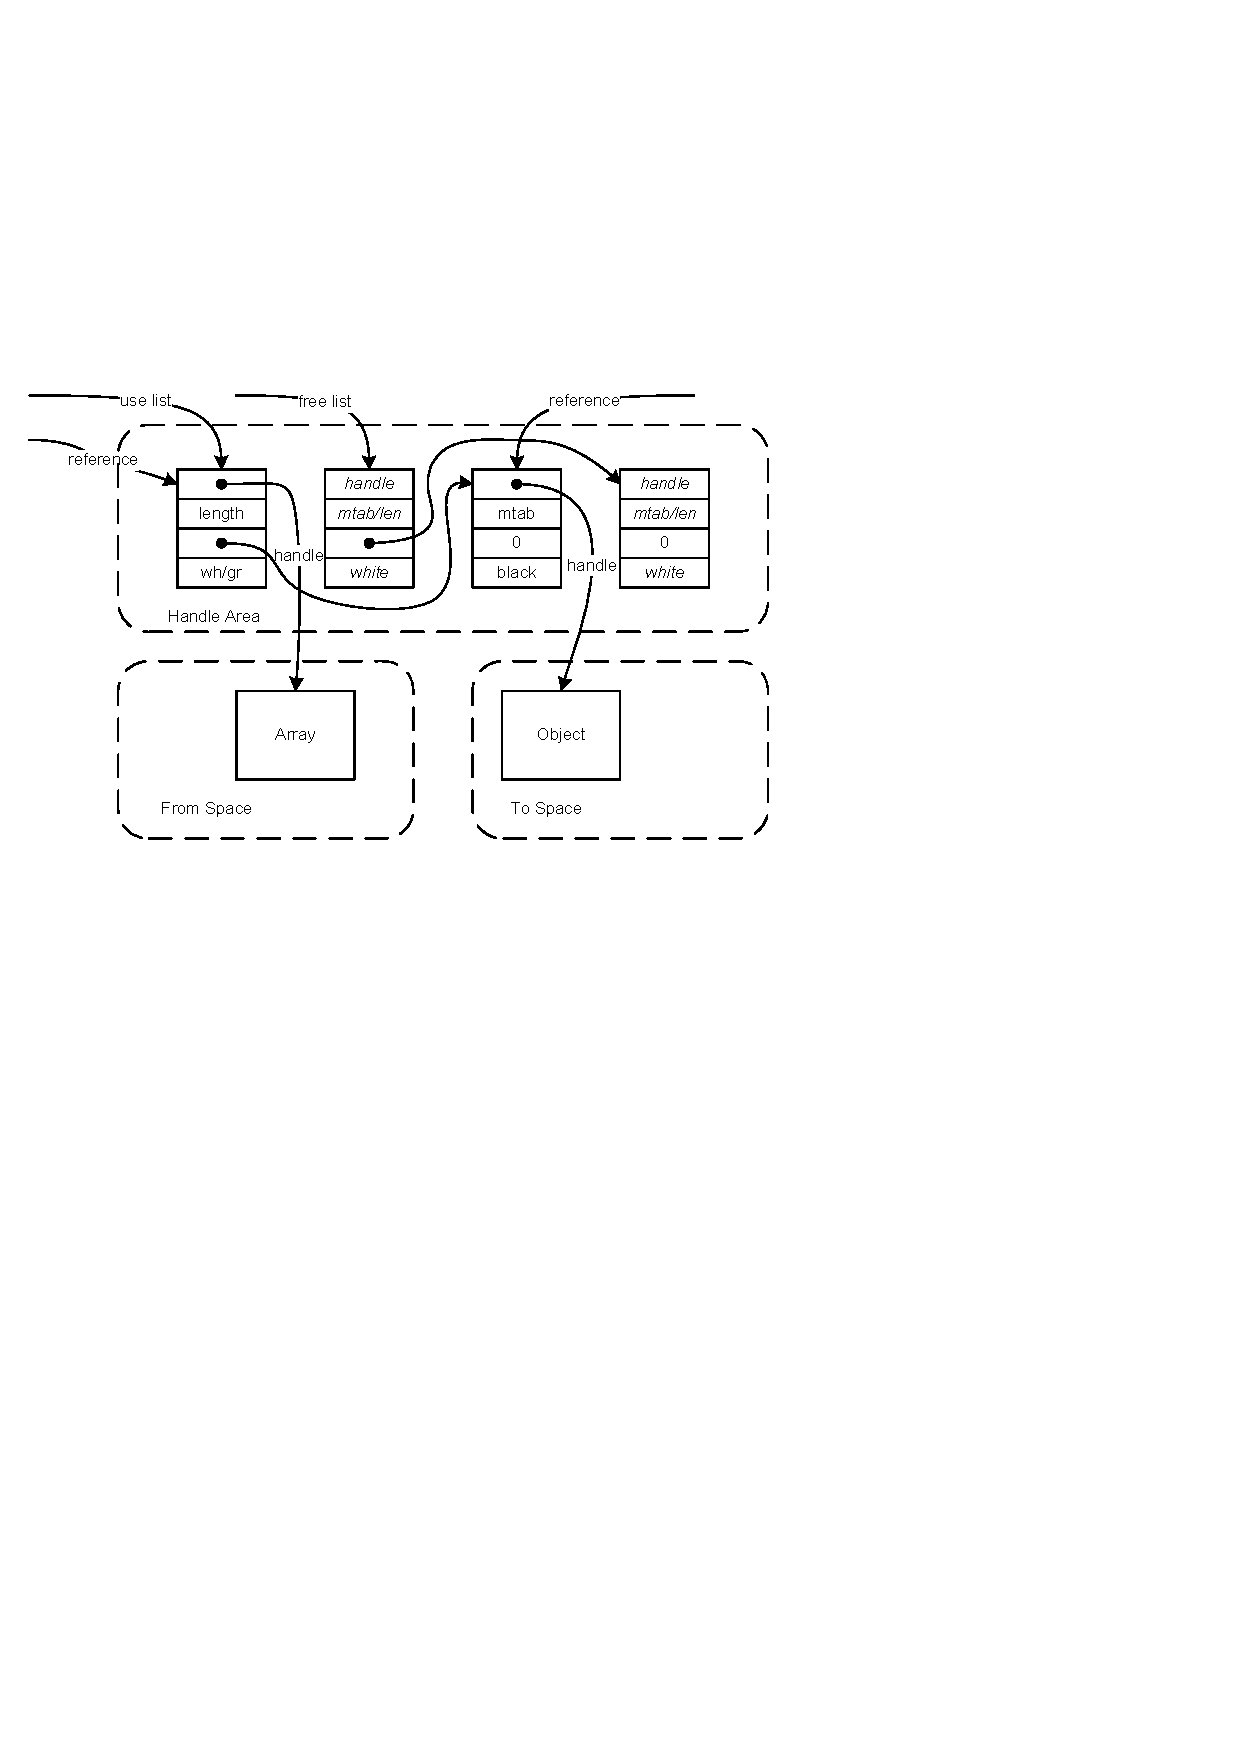
\includegraphics{jvm/handles}
  \caption{Heap layout with the handle area}\label{fig:handles}
\end{figure*}

To simplify object move by the collector, all objects are accessed
with one indirection, called the handle. The handle also contains
auxiliary object data structures, such as a pointer to the method
table or the array length. Instead of Baker's read barrier we have an
additional mark stack which is a threaded list within the handle
structure. An additional field (as shown in Figure~\ref{fig:handles})
in the handle structure is used for a free list and a use list of
handles.

The indirection through a handle, although a very light-weight read
barrier, is usually still considered as a high overhead. Metronome
\cite{gc:bacon03} uses a forwarding pointer as part of the object and
performs forwarding \emph{eagerly}. Once the pointer is forwarded,
subsequent uses of the reference can be performed on the direct
pointer until a GC preemption point. This optimization is performed
by the compiler.

JOP uses a hardware based optimization for this indirection
\cite{jop:oohw:jtres2007}. The indirection is unconditionally
performed in the memory access unit. Furthermore, null pointer checks
and array bounds checks are done in parallel to this indirection.

There are two additional benefits from an explicit handle area instead of a
forwarding pointer: (a) access to the method table or array size needs no
indirection, and (b) the forwarding pointer and the auxiliary data
structures do not need to be copied by the GC.

The fixed handle area is not subject to fragmentation as all handles
have the same size and are recycled at a sweep phase with a simple
free list. However, the reserved space has to be sized (or the GC
period adapted) for the maximum number of objects that are live or
are floating garbage.


\subsection{The Collector}

The collector can operate in two modes: (1) as stop-the-world
collector triggered on allocation when the heap is full, or (2) as
concurrent real-time collector running in its own thread.

The real-time collector is scheduled periodically at the lowest
priority and within each period it performs the following steps:
\begin{description}
    \item[Flip] An atomic flip exchanges the roles of tospace and
    fromspace.
    \item[Mark roots] All static references are pushed onto the mark
    stack. Only a single push operation needs to be atomic. As the
    thread stacks are empty we do not need an atomic scan of thread
    stacks.
    \item[Mark and copy] An object is popped from the mark stack,
    all referenced objects, which are still white, are pushed on the
    mark stack, the object is copied to tospace and the handle
    pointer is updated.
    \item[Sweep handles] All handles in the use list are checked if
    they still point into tospace (black objects) or can be added to
    the handle free list.
    \item[Clear fromspace] At the end of the collector work the
    fromspace that contains only white objects is initialized with
    zero. Objects allocated in that space (after the next flip) are
    already initialized and allocation can be performed in constant
    time.
\end{description}
%
To reduce blocking time, a hardware unit performs copies of objects
and arrays in an interruptible fashion, and records the copy position
on an interrupt. On an object or array access the hardware knows
whether the access should go to the already copied part in the
tospace or in the not yet copied part in the fromspace. It has to be
noted that splitting larger arrays into smaller chunks, as done in
Metronome~\cite{gc:bacon03} and in the GC for the
JamaicaVM~~\cite{gc:siebert:phd}, is a software option to reduce the
blocking time.

The collector has two modes of operation: one for the initialization
phase and one for the mission phase. At the initialization phase it
operates in a stop-the-world fashion and gets invoked when a memory
request cannot be satisfied. In this mode the collector scans the
stack of the single thread conservatively. It has to be noted that
each reference points into the handle area and not to an arbitrary
position in the heap. This information is considered by the GC to
distinguish pointers from primitives. Therefore the chance to keep an
object artificially alive is low.

%% This is RTS paper stuff and should go away in the handbook
As part of the mission start one stop-the-world cycle is performed to
clean up the heap from garbage generated at initialization. From that
point on the GC runs in concurrent mode in its own thread and omits
scanning of the thread stacks.

\subsubsection{Implementation Code Snippets}

This sections shows the important code fragments of the
implementation. As can be seen, the implementation is quite short.

\paragraph{Flip} involves manipulation of a few pointers and changes
the meaning of black (\code{toSpace}) and white.
%
\begin{lstlisting}
    synchronized (mutex) {
        useA = !useA;
        if (useA) {
            copyPtr = heapStartA;
            fromSpace = heapStartB;
            toSpace = heapStartA;
        } else {
            copyPtr = heapStartB;
            fromSpace = heapStartA;
            toSpace = heapStartB;
        }
        allocPtr = copyPtr+semi_size;
    }
\end{lstlisting}


\paragraph{Root Marking} When the GC runs in concurrent mode only
the static reference fields form the root set and are scanned. The
stop-the-world mode of the GC also scans all stacks from all
threads.
%
\begin{lstlisting}
    int addr = Native.rdMem(addrStaticRefs);
    int cnt = Native.rdMem(addrStaticRefs+1);
    for (i=0; i<cnt; ++i) {
        push(Native.rdMem(addr+i));
    }
\end{lstlisting}

\paragraph{Push} All gray objects are pushed on a gray stack. The
gray stack is a list threaded within the handle structure.
%
\begin{lstlisting}
    if (Native.rdMem(ref+OFF_GREY)!=0) {
        return;
    }
    if (Native.rdMem(ref+OFF_GREY)==0) {
        // pointer to former gray list head
        Native.wrMem(grayList, ref+OFF_GREY);
        grayList = ref;
    }
\end{lstlisting}

\paragraph{Mark and Copy} The following code snippet shows the
central GC loop.
%
\begin{lstlisting}
    for (;;) {

        // pop one object from the gray list
        synchronized (mutex) {
            ref = grayList;
            if (ref==GREY_END) {
                break;
            }
            grayList = Native.rdMem(ref+OFF_GREY);
            // mark as not in list
            Native.wrMem(0, ref+OFF_GREY);
        }

        // push all childs
        // get pointer to object
        int addr = Native.rdMem(ref);
        int flags = Native.rdMem(ref+OFF_TYPE);
        if (flags==IS_REFARR) {
            // is an array of references
            int size = Native.rdMem(ref+OFF_MTAB_ALEN);
            for (i=0; i<size; ++i) {
                push(Native.rdMem(addr+i));
            }
        } else if (flags==IS_OBJ){
            // its a plain object
            // get pointer to method table
            flags = Native.rdMem(ref+OFF_MTAB_ALEN);
            // get real flags
            flags = Native.rdMem(flags+MTAB2GC_INFO);
            for (i=0; flags!=0; ++i) {
                if ((flags&1)!=0) {
                    push(Native.rdMem(addr+i));
                }
                flags >>>= 1;
            }
        }

        // now copy it - color it BLACK
        int size = Native.rdMem(ref+OFF_SIZE);
        synchronized (mutex) {
            // update object pointer to the new location
            Native.wrMem(copyPtr, ref+OFF_PTR);
            // set it BLACK
            Native.wrMem(toSpace, ref+OFF_SPACE);
            // copy it
            for (i=0; i<size; ++i) {
                Native.wrMem(Native.rdMem(addr+i), copyPtr+i);
            }
            copyPtr += size;
        }
    }
\end{lstlisting}

\paragraph{Sweep Handles} At the end of the mark and copy phase the
handle area is swept to find all unused handles (the one that still
point into \code{fromSpace}) and add them to the free list.
%
\begin{lstlisting}
    synchronized (mutex) {
        ref = useList;      // get start of the list
        useList = 0;        // new uselist starts empty
    }

    while (ref!=0) {

        int next = Native.rdMem(ref+OFF_NEXT);
        // a BLACK one
        if (Native.rdMem(ref+OFF_SPACE)==toSpace) {
            // add to used list
            synchronized (mutex) {
                Native.wrMem(useList, ref+OFF_NEXT);
                useList = ref;
            }
        // a WHITE one
        } else {
            // add to free list
            synchronized (mutex) {
                Native.wrMem(freeList, ref+OFF_NEXT);
                freeList = ref;
                Native.wrMem(0, ref+OFF_PTR);
            }
        }
        ref = next;
    }
\end{lstlisting}

\paragraph{Clear Fromspace} The last step of the GC clears the
fromspace to provide a constant time allocation after the next flip.
%
\begin{lstlisting}
        for (int i=fromSpace; i<fromSpace+semi_size; ++i) {
            Native.wrMem(0, i);
        }
\end{lstlisting}

\subsection{The Mutator}

The coordination between the mutator and the collector is performed
within the \code{new} and \code{newarray} bytecodes and within write
barriers for JVM bytecodes \code{putfield} and \code{putstatic} for
reference fields, and bytecode \code{aastore}. The field access
bytecodes are substituted at application link time (run of
\code{JOPizer}). Only write accesses to reference fields are
substituted by special versions of the bytecodes
(\code{putfield\_ref} and \code{putstatic\_ref}). Therefore, the
write barrier code is only executed on reference write access.

\subsubsection{Allocation}

Objects are allocated black (in tospace). In non real-time collectors
it is more common to allocate objects white. It is argued
\cite{gc:dijkstra78} that objects die young and the chances are high
that the GC never needs to touch them. However, in the worst case no
object that is created and becomes garbage during the GC cycle can be
reclaimed. Those floating garbage will be reclaimed in the next GC
cycle. Therefore, we do not benefit from the white allocation
optimization in a real-time GC. Allocating a new object black has the
benefit that those objects do not need to be copied. The same
argument applies to the chosen write barrier. The code in
Listing~\ref{lst:new} shows the simple implementation of bytecode
\code{new}:

\begin{lstlisting}[float=t, caption={Implementation of bytecode \code{new} in JOP�s JVM},
label=lst:new]

synchronized (GC.mutex) {
    // we allocate from the upper part
    allocPtr -= size;
    ref = getHandle(size);
    // mark as object
    Native.wrMem(IS_OBJ, ref+OFF_TYPE);
    // pointer to method table in the handle
    Native.wrMem(cons+CLASS_HEADR, ref+OFF_MTAB_ALEN);
}
\end{lstlisting}

As the old fromspace is cleared by the GC, the new object is already
initialized and \code{new} executes in constant time. The methods
\code{Native.rdMem()} and \code{Native.wrMem()} provide direct access
to the main memory. Only those two native methods are necessary for
an implementation of a GC in pure Java.

\subsubsection{Write Barriers}

For a concurrent (incremental) GC some coordination between the
collector and the mutator are necessary. The usual solution is a
write barrier in the mutator to not foil the collector. According to
\cite{gc:wils94} GC concurrent algorithms can be categorized into:

\begin{description}
    \item[Snapshot-at-beginning] Keep the object graph as it was at
    the the GC start
    \begin{itemize}
        \item Save the to-be-overwritten reference
        \item More conservative -- not an issue for RTs as worst case
        counts
        \item Allocate black
        \item New objects (e.g.\ new stack frames) do not need a
        write barrier
        \item Optimization: with atomic root scan of the thread
        stacks no write barrier is necessary for locals and the JVM
        stack
    \end{itemize}
    \item[Incremental update] \emph{Help} the GC by doing some collection
    work in the mutator
    \begin{itemize}
        \item Preserve strong tri-color invariant (no pointer from
        black to white objects)
        \item On black to white shade the white object (shade the
        black is unusual)
        \item Allocate black (in contrast to \cite{gc:dijkstra78})
        \item Needs write barriers for locals and manipulation on
        the stack
        \item Less conservative than snapshot-at-beginning
    \end{itemize}
\end{description}

The usual choice is snapshot-at-beginning with atomic root scan of
all thread stacks to avoid write barriers on locals. Assume the
following assignment of a reference:
\begin{lstlisting}
    o.r = ref;
\end{lstlisting}
There are three references involved that can be manipulated:
\begin{itemize}
    \item The old value of \code{o.r}
    \item The new value \code{ref}
    \item The object \code{o}
\end{itemize}
The three possible write barriers are:
\begin{enumerate}
    \item
Snapshot-at-beginning/weak tri-color invariant:
\begin{lstlisting}
    if (white(o.r)) markGrey(o.r);
    o.r = ref;
\end{lstlisting}
    \item
Incremental/strong tri-color invariant with push forward
\begin{lstlisting}
    if (black(o) && white(ref)) markGrey(ref);
    o.r = ref;
\end{lstlisting}
This barrier can be optimized to only check if \code{ref} is white.

    \item
Incremental/strong tri-color invariant with push back
\begin{lstlisting}
    if (black(o) && white(ref)) markGrey(o);
    o.r = ref;
\end{lstlisting}

\end{enumerate}

We have no stack roots when the collector runs. Therefore we could
use the incremental write barrier for object fields only. However,
for the worst case all floating garbage will not be found by the GC
in the current cycle. Therefore, we use the snapshot-at-begin write
barrier in our implementation.

A snapshot-at-beginning write-barrier synchronizes the mutator with
the collector on a reference store into a static field, an object
field, or an array. The \emph{to be overwritten} field is shaded gray
as shown in Listing~\ref{lst:barrier}. An object is shaded gray by
pushing the reference of the object onto the mark
stack.\footnote{Although the GC is a copying collector a mark stack
is needed to perform the object copy in the GC thread and not by the
mutator.} Further scanning and copying into tospace -- coloring it
black -- is left to the GC thread. One field in the handle area is
used to implement the mark stack as a simple linked list.
Listing~\ref{lst:barrier} shows the implementation of \code{putfield}
for reference fields.

\begin{lstlisting}[float=t, caption={Snapshot-at-beginning write-barrier in JOP�s JVM},
label=lst:barrier]

private static void f_putfield_ref(int ref, int value, int index) {

    synchronized (GC.mutex) {

        // snapshot-at-beginning barrier
        int oldVal = Native.getField(ref, index);
        // Is it white?
        if (oldVal != 0
            && Native.rdMem(oldVal+GC.OFF_SPACE) != GC.toSpace) {
            // Mark grey
            GC.push(oldVal)
        }
        Native.putField(ref, index, value);
    }
}
\end{lstlisting}

%All \code{putfield} bytecodes are replaced by quick variants on class
%linking. During this step also \code{putfield} instructions for
%references and double-word length fields (\code{double} and
%\code{long}) are replaced by special bytecodes. Therefore, the code
%shows the special bytecode \code{putfield\_ref}.

Note that field and array access is implemented in hardware on JOP.
Only write accesses to reference fields need to be protected by the
write-barrier, which is implemented in software. During class linking
all write operations to reference fields (\code{putfield} and
\code{putstatic} when accessing reference fields) are replaced by a
JVM internal bytecodes (e.g., \code{putfield\_ref}) to execute the
write-barrier code as shown before.
% RTS version
% in Figure~\ref{fig:barrier}.
The shown code is part of a special class
(\code{com.jopdesign.sys.JVM}) where Java bytecodes that are not
directly implemented by JOP can be implemented in Java
\cite{jop:thesis}. %% add a reference to a Section in the handbook.

The methods of class \code{Native} are JVM internal methods needed to
implement part of the JVM in Java. The methods are replaced by
regular or JVM internal bytecodes during class linking. Methods
\code{getField(ref, index)} and \code{putField(ref, value, index)}
map to the JVM bytecodes \code{getfield} and \code{putfield}. The
method \code{rdMem()} is an example of an internal JVM bytecode and
performs a memory read. The null pointer check for
\code{putfield\_ref} is implicitly performed by the hardware
implementation of \code{getfield} that is executed by
\code{Native.getField()}. The hardware implementation of
\code{getfield} triggers an exception interrupt when the reference is
null. The implementation of the write-barrier shows how a bytecode is
substituted by a special version (\code{pufield\_ref}), but uses in
the software implementation the hardware implementation of that
bytecode (\code{Naitve.putfield()}).

In principle this write-barrier could also be implemented in
microcode to avoid the expensive invoke of a Java method. However,
the interaction with the GC, which is written in Java, is simplified
by the Java implementation. As a future optimization we intend to
inline the write-barrier code.

The collector runs in its own thread and the priority is assigned
according to the deadline, which equals the period of the GC cycle.
As the GC period is usually longer than the mutator task deadlines,
the GC runs at the lowest priority. When a high priority task becomes
ready, the GC thread will be preempted. Atomic operations of the GC
are protected simply by turning the timer interrupt off.\footnote{If
interrupt handlers are allowed to change the object graph those
interrupts also need to be disabled.} Those atomic sections lead to
release jitter of the real-time tasks and shall be minimized. It has
to be noted that the GC protection with interrupt disabling is not an
option for multiprocessor systems.

\section{Evaluation}

To evaluate the proposed real-time GC we execute a simple test
application on JOP and measure heap usage and the release time jitter
of high priority threads. The test setup consists of JOP implemented
in an Altera Cyclone FPGA clocked at 100~MHz. The main memory is a
1~MB SRAM with an access time of two clock cycles. JOP is configured
with a 4~KB method cache (a special form of instruction cache) and a
128 entry stack cache. No additional data cache is used.

\subsection{Scheduling Experiments}

In this section we test an implementation of the concurrent-copy
garbage collector on JOP. The tests are intended to get some
confidence that the formulas for the collector periods are correct.
Furthermore we visualize the actual heap usage of a running system.

The examples are synthetic benchmarks that emulate worst-case
execution time (WCET) by executing a busy loop after allocation of
the data. The WCET of the collector was measured to be 10.4~ms when
executing it with scheduling disabled during one collection cycle for
example 1 and 11.2~ms for example 2. We use 11~ms and 12~ms
respectively as the WCET of the collector for the following
examples\footnote{It has to be noted that measuring execution time is
not a safe method to estimate WCET values.}.


Listing~\ref{lst:excode} shows our worker thread with the busy loop.
The data is allocated at the start of the period and freed after the
simulated execution. \code{waitForNextPeriod} blocks until the next
release time for the periodic thread.

\begin{lstlisting}[float, caption={Example periodic thread with a busy loop},
label=lst:excode]
    public void run() {

        for (;;) {
            int[] n = new int[cnt];
            // simulate work load
            busy(wcet);
            n = null;
            waitForNextPeriod();
        }
    }

    final static int MIN_US = 10;

    static void busy(int us) {

        int t1, t2, t3;
        int cnt;

        cnt = 0;
        // get the current time in us
        t1 = Native.rd(Const.IO_US_CNT);

        for (;;) {
            t2 = Native.rd(Const.IO_US_CNT);
            t3 = t2-t1;
            t1 = t2;
            if (t3<MIN_US) {
                cnt += t3;
            }
            if (cnt>=us) {
                return;
            }
        }
    }
\end{lstlisting}

For the busy loop to simulate \emph{real} execution time, and not
elapsed time, the constant \code{MIN\_US} has to be less than the
time for two context switches, but larger than the execution time of
one iteration of the busy loop. In this case only cycles executed by
the busy loop are counted for the execution time and interruption
due to a higher priority thread is not part of the execution time
measurement.

In our example we use a concurrent-copy collector with a heap size
(for both semi-spaces) of 100~KB. At startup the JVM allocates about
3.5~KB data. We incorporate\footnote{The suggested handling of static
data to be moved to \emph{immortal} memory at mission start is not
yet implemented.} these 3.5~KB as static live data $L_s$.



\subsubsection{Independent Threads}

The first example consists of two threads with the properties listed
in Table~\ref{fig:ex1}. $T_i$ is the period, $C_i$ the WCET, and
$a_i$ the maximum amount of memory allocated each period. Note that
the period for the collector thread is also listed in the table
although it is a result of the worker thread properties and the heap
size.

\begin{table}[tb]
\begin{center}
\begin{tabular}{lrrr}
    \toprule
    & \multicolumn{1}{c}{$T_i$} & \multicolumn{1}{c}{$C_i$} & \multicolumn{1}{c}{$a_i$} \\
    \midrule
    $\tau_1$ & 5 ms & 1 ms & 1 KB \\
    $\tau_2$ & 10 ms & 3 ms & 3 KB \\
    $\tau_{GC}$ & 77 ms & 11 ms & \\
    \bottomrule
\end{tabular}
    \caption{Thread properties for experiment 1}
\label{fig:ex1}
\end{center}
\end{table}

With the periods $T_i$ and the memory consumption $a_i$ for the two
worker threads we calculate the maximum period $T_{GC}$ for the
collector thread $\tau_{GC}$ by using Theorem~\ref{sch:theorem}
\begin{align*}
    T_{GC} & \le \frac{H_{CC}-2\left(L_s+\sum_{i=1}^{n} a_i\right)-2\sum_{i=1}^{n} a_i}
        {2\sum_{i=1}^{n} \frac{a_i}{Ti}} \\
           & \le \frac{100-2(3.5+4)-2\cdot4}
           {2\left(\frac{1}{5}+\frac{3}{10}\right)}\mbox{ms}\\
           & \le 77\mbox{ms}
\end{align*}

The priorities are assigned rate-monotonic \cite{321743} and we
perform a quick schedulability check with the periods $T_i$ and the
WCETs $C_i$ by calculation of the processor utilization $U$ for all
three threads
\begin{align*}
    U & = \sum_{i=1}^{3}\left(\frac{C_i}{T_i}\right)\\
      & = \frac{1}{5} + \frac{3}{10} + \frac{11}{77}\\
      & = 0.643
\end{align*}
which is less than the maximum utilization for three tasks
\begin{align*}
    U_{max} & = m*(2^{\frac{1}{m}}-1)\\
      & = 3*(2^{\frac{1}{3}}-1)\\
      & \approx 0.78
\end{align*}

In Figure~\ref{fig:ex1:mem} the memory trace for this system is
shown.
\begin{figure}
\begin{center}
    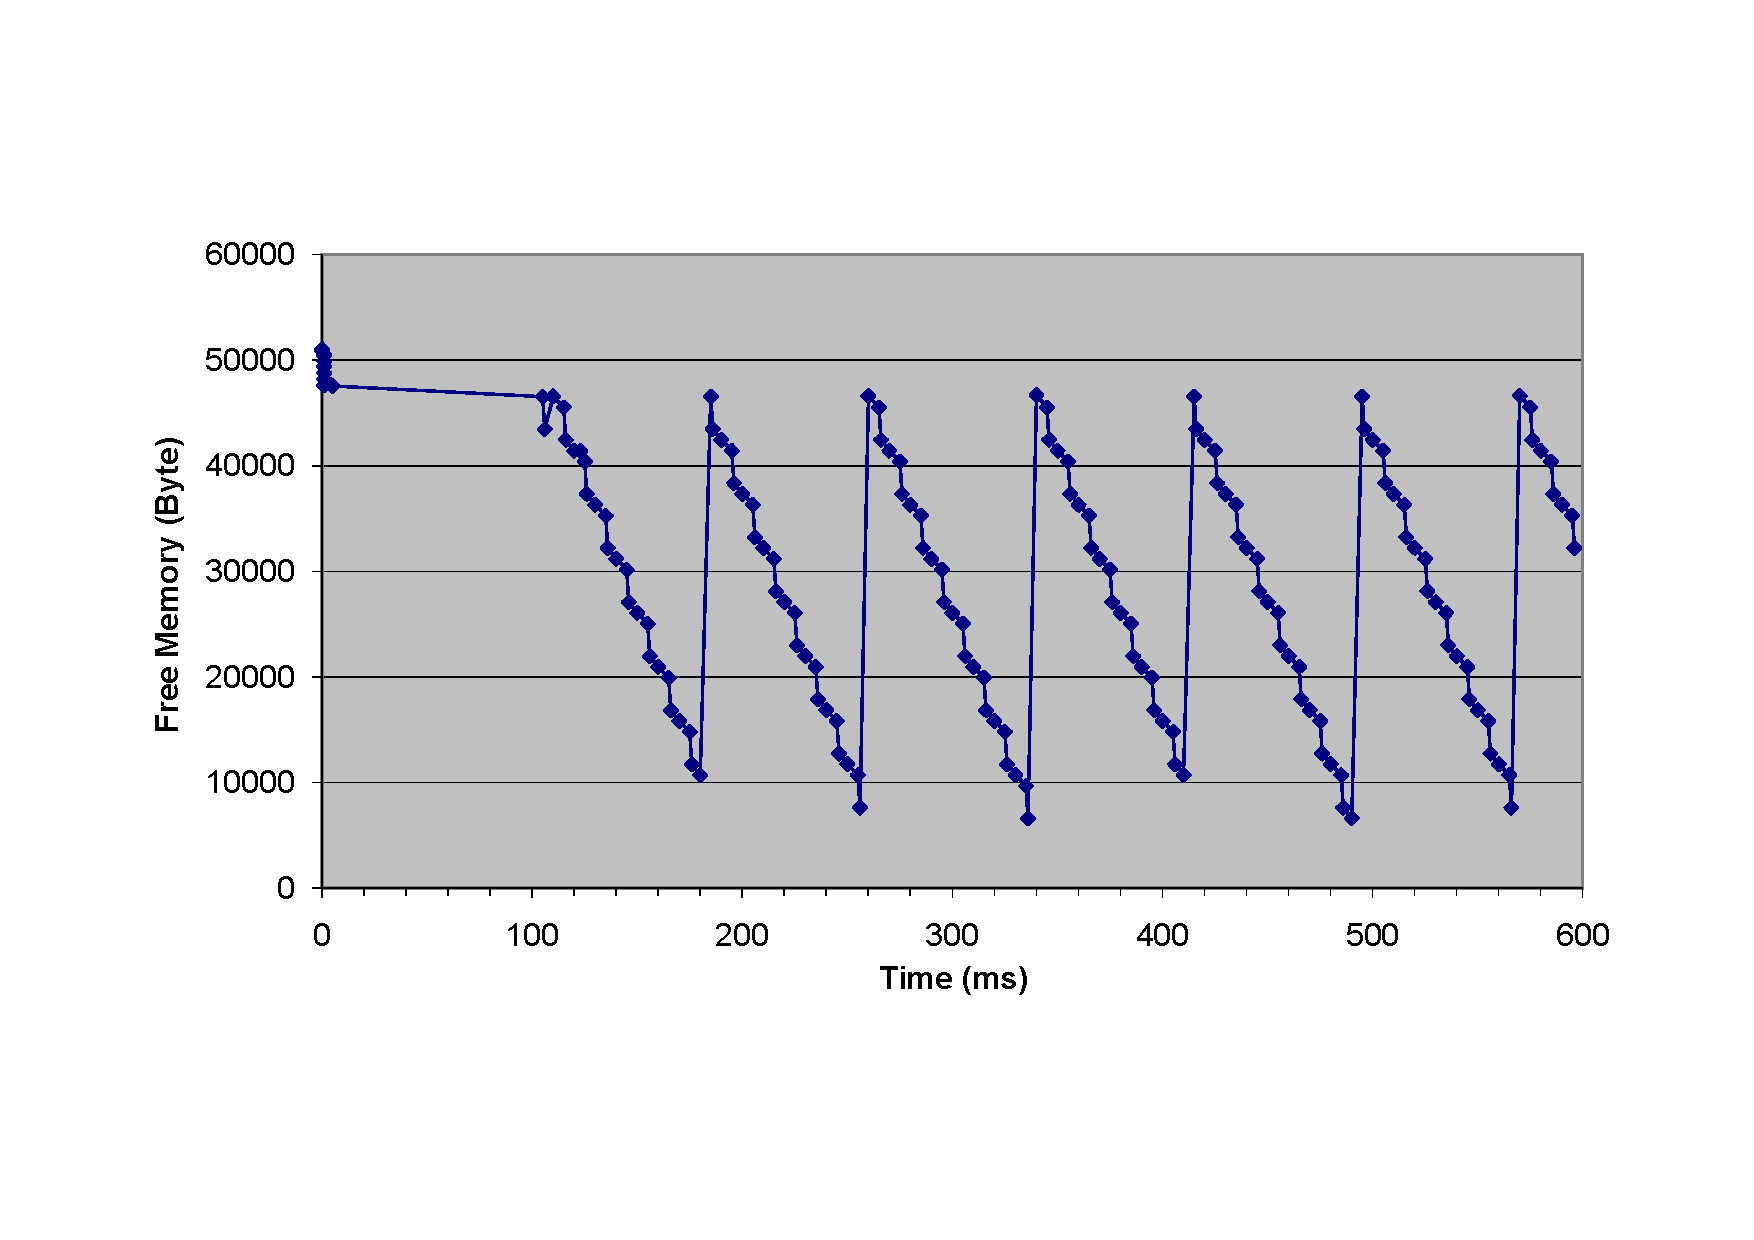
\includegraphics[width=\excelwidth]{jvm/gc_ex1}
    \caption{Free memory in experiment 1}
\label{fig:ex1:mem}
\end{center}
\end{figure}
The graph shows the free memory in one semi-space (the to-space,
which is 50~KB) during the execution of the application. The
individual points are recorded with time-stamps at the end of each
allocation request.

In the first milliseconds we see allocation requests that are part
of the JVM startup (most of it is static data). The change to the
mission phase is delayed 100~ms and the first allocation from a
periodic thread is at 105~ms. The collector thread also starts at
the same time and the first semi-space flip can be seen at 110~ms
(after one allocation from each worker thread). We see the 77~ms
period of the collector in the jumps in the free memory graph after
the flip. The different memory requests of two times 1~KB from
thread $\tau_1$ and one time 3~KB from thread $\tau_2$ can be seen
every 10~ms.

In this example the heap is used until it is almost full, but the
application never runs out of memory and no thread misses a deadline.
From the regular allocation pattern we also see that this collector
runs concurrently. With a stop-the-world collector we would notice
gaps of 10~ms (the measured execution time of the collector) in the
graph.

\subsubsection{Producer/Consumer Threads}

For the second experiment we split our thread $\tau_1$ to a producer
thread $\tau_1$ and a consumer thread $\tau_3$ with a period of
30~ms. We assume after the split that the producer's WCET is halved
to 500~us. The consumer thread is assumed to be more efficient when
working on lager blocks of data than in the former example
($C_3$=2~ms instead of 6*500~$\mu$s). The rest of the setting
remains the same (the worker thread $\tau_2$). Table~\ref{fig:ex2}
shows the thread properties for the second experiment.

\begin{table}[tb]
\begin{center}
\begin{tabular}{lrrr}
    \toprule
    & \multicolumn{1}{c}{$T_i$} & \multicolumn{1}{c}{$C_i$} &\multicolumn{1}{c}{$a_i$} \\
    \midrule
    $\tau_1$ & 5 ms & 0.5 ms & 1 KB \\
    $\tau_2$ & 10 ms & 3 ms & 3 KB \\
    $\tau_3$ & 30 ms & 2 ms & \\
    $\tau_{GC}$ & 55 ms & 12 ms & \\
    \bottomrule
\end{tabular}
    \caption{Thread properties for experiment 2}
\label{fig:ex2}
\end{center}
\end{table}

As explained in Section~\ref{sec:prod:cons} we calculate the
lifetime factor $l_1$ for memory allocated by the producer $\tau_1$
with the corresponding consumer $\tau_3$ with period $T_3$.
\begin{equation*}
    l_1 = \left\lceil\frac{2 T_3}{T_1}\right\rceil
        = \left\lceil\frac{2 \times 30}{5}\right\rceil
        = 12
\end{equation*}
%
The maximum collector period $T_{GC}$ is
\begin{align*}
    T_{GC} & \le \frac{H_{CC}-2\left(L_s+\sum_{i=1}^{n} a_i l_i\right)-2\sum_{i=1}^{n} a_i}
        {2\sum_{i=1}^{n} \frac{a_i}{Ti}} \\
           & \le \frac{100-2(3.5+1\cdot12+3+0)-2\cdot4}
           {2\left(\frac{1}{5}+\frac{3}{10}+\frac{0}{30}\right)}\mbox{ms}\\
           & \le 55\mbox{ms}
\end{align*}
We check the maximum processor utilization:
\begin{align*}
    U & = \sum_{i=1}^{4}\left(\frac{C_i}{T_i}\right)\\
      & = \frac{0.5}{5} + \frac{3}{10} + \frac{2}{30} + \frac{12}{55}\\
      & = 0.685 \le 4*(2^{\frac{1}{4}}-1) \approx 0.76
\end{align*}

In Figure~\ref{fig:ex2:mem} the memory trace for the system with one
producer, one consumer, and one independent thread is shown.
\begin{figure}
\begin{center}
    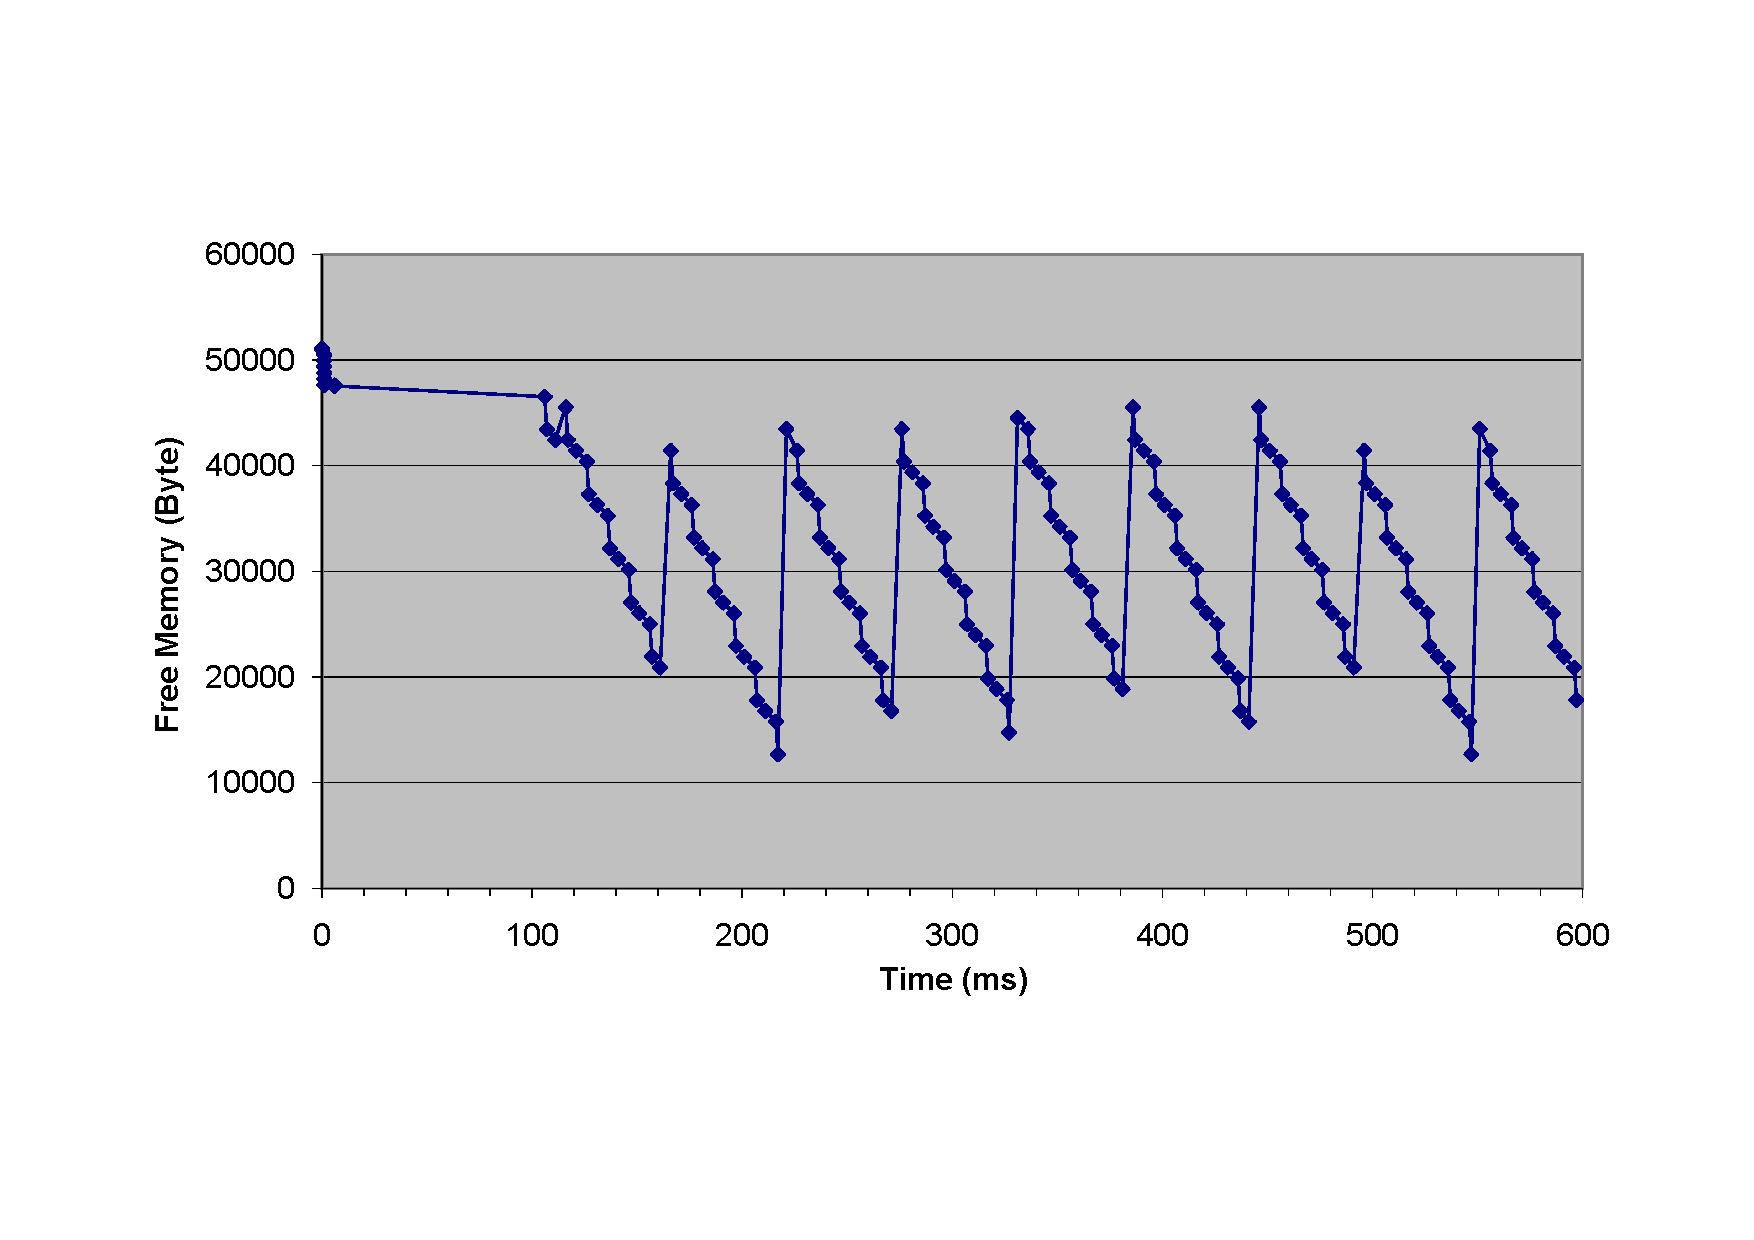
\includegraphics[width=\excelwidth]{jvm/gc_ex2}
    \caption{Free memory in experiment 2}
\label{fig:ex2:mem}
\end{center}
\end{figure}
%
Again, we see the 100~ms delayed mission start after the startup and
initialization phase, in this example at about 106~ms. Similar to
the former example the first collector cycle performs the flip a few
milliseconds after the mission start. We see the shorter collection
period of 55~ms. The allocation pattern (two times 1~KB and one time
3~KB per 10~ms) is the same as in the former example as the threads
that allocate the memory are still the same.

We have also run this experiment for a longer time than shown in
Figure~\ref{fig:ex2:mem} to see if we find a point in the execution
trace where the remaining free memory is less than the value at
217~ms. The pattern repeats and the observed value at 217~ms is the
minimum.




\subsection{Measuring Release Jitter}

%% TODO use text and new results form JTRES/TECS paper.

Our main concern on garbage collection in real-time systems is the
blocking time introduced  by the GC due to atomic code sections.
This blocking time will be seen as release time jitter on the
real-time threads. Therefore we want to measure this jitter.

\begin{lstlisting}[float=t, caption={Measuring release time jitter},
label=lst:measure]

public boolean run() {

    int t = Native.rdMem(Const.IO_US_CNT);
    if (!notFirst) {
        expected = t+period;
        notFirst = true;
    } else {
        int diff = t-expected;
        if (diff>max) max = diff;
        if (diff<min) min = diff;
        expected += period;
    }
    work();

    return true;
}
\end{lstlisting}

Listing~\ref{lst:measure} shows how we measure the jitter. Method
\code{run()} is the main method of the real-time thread and executed
on each periodic release. Within the real-time thread we have no
notion about the start time of the thread. As a solution we measure
the actual time on the first iteration and use this time as first
release time. In each iteration the expected time, stored in the
variable \code{expected}, is incremented by the \code{period}. In
each iteration (except the first one) the actual time is compared
with the expected time and the maximum value of the difference is
recorded.

As noted before, we have no notion about the \emph{correct} release
times. We measure only relative to the first release. When the first
release is delayed (due to some startup code or interference with a
higher priority thread) we have a positive offset in
\code{expected}. On an exact release in a later iteration the time
difference will be negative (in \code{diff}). Therefore, we also
record the minimum value for the difference between the actual time
and the expected time. The maximum measured release jitter is the
difference between \code{max} and \code{min}.

To provide a baseline we measure the release time jitter of a single
real-time thread (plus an endless loop in the \code{main} method as
an idle non-real-time background thread). No GC thread is scheduled.
The code is similar to the code in Listing~\ref{lst:measure}. A stop
condition is inserted that prints out the minimum and maximum time
differences measured after 1 million iterations.

\begin{table}
    \centering
    \begin{tabular}{rr}
    \toprule
    Period & Jitter \\
    \midrule
    200 $\mu$s & 0 $\mu$s \\
    100 $\mu$s & 0 $\mu$s \\
    50 $\mu$s & 17 $\mu$s \\
    \bottomrule
    \end{tabular}
    \caption{Release jitter for a single thread}
    \label{tab:single}
\end{table}

Table~\ref{tab:single} shows the measured jitter for different
thread periods. We observed no jitter for periods of 100~$\mu$s and
longer. At a period of 50~$\mu$s the scheduler introduces a
considerable amount of jitter. From this measurement we conclude
that 100~$\mu$s is the practical shortest period we can handle with
our system. We will use this period for the high-priority real-time
thread in the following measurement with an enabled GC.

\subsection{Measurements}

%% TODO use new results form JTRES/TECS paper.

The test application consisting of three real-time threads
($\tau_{hf}$, $\tau_{p}$, and $\tau_{c}$), one logging thread
$\tau_{log}$, and the GC thread $\tau_{gc}$. All three real-time
threads measure the difference between the expected release time and
the actual release time (as shown in Figure~\ref{lst:measure}). The
minimum and maximum values are recorded and regularly printed to the
console by the logging thread $\tau_{log}$. Table~\ref{tab:exp}
shows the release parameters for the five threads. Priority is
assigned deadline monotonic. Note that the GC thread has a shorter
period than the logger thread, but a longer deadline. For our
approach to work correctly the GC thread \emph{must} have the lowest
priority. Therefore all other threads with a longer period than the
GC thread must be assigned a shorter deadline.

\begin{table}
    \centering
    \begin{tabular}{lrrr}
    \toprule
    Thread & Period & Deadline & Priority \\
    \midrule
    $\tau_{hf}$ & 100 $\mu$s & 100 $\mu$s & 5 \\
    $\tau_{p}$ &  1 ms & 1 ms & 4 \\
    $\tau_{c}$ & 10 ms & 10 ms & 3 \\
    $\tau_{log}$ & 1000 ms & 100 ms & 2 \\
    $\tau_{gc}$ & 200 ms & 200 ms & 1 \\
    \bottomrule
    \end{tabular}
    \caption{Thread properties of the test program}
    \label{tab:exp}
\end{table}

Thread $\tau_{hf}$ represents a high-frequency thread without
dynamic memory allocation. This thread should observe minimal
disturbance by the GC thread.

The threads $\tau_{p}$ and $\tau_{c}$ represent a producer/consumer
pair that uses dynamically allocated memory for communication. The
producer appends the data at a frequency of 1~kHz to a simple list.
The consumer thread runs at 100~Hz and processes all currently
available data in the list and removes them from the list. The
consumer will process between 9 and 11 elements (depending on the
execution time of the consumer and the thread phasing).

It has to be noted that this simple and common communication pattern
cannot be implemented with the scoped memory model of the RTSJ.
First, to use a scope for communication, we have to keep the scope
alive with a \emph{wedge} thread \cite{conf/isorc/PizloFHV04} when
data is added by the producer. We would need to notify this wedge
thread by the consumer when all data is consumed. However, there is
no single instant available where we can \emph{guarantee} that the
list is empty. A possible solution for this problem is described in
\cite{conf/isorc/PizloFHV04} as \emph{handoff} pattern. The pattern
is similar to double buffering, but with an explicit copy of the
data. The elegance of a simple list as buffer queue between the
producer and the consumer is lost.

Thread $\tau_{log}$ is not part of the real-time systems simulated
application code. Its purpose is to print the minimum and maximum
differences between the measured and expected release times (see
former section) of threads $\tau_{hf}$ and $\tau_{p}$ to the console
periodically.

Thread $\tau_{gc}$ is a standard periodic real-time thread executing
the GC logic. The GC thread period was chosen quite short in that
example. A period in the range of seconds would be enough for the
memory allocation by $\tau_{p}$. However, to stress the interference
between the GC thread and the application threads we artificially
shortened the period.

\begin{table}
    \centering
    \begin{tabular}{lr}
    \toprule
    Threads & Jitter \\
    \midrule
    $\tau_{hf}$ & 0 $\mu$s \\
    $\tau_{hf}$, $\tau_{log}$ & 7 $\mu$s \\
    $\tau_{hf}$, $\tau_{log}$,$\tau_{p}$,$\tau_{c}$ & 14 $\mu$s \\
    $\tau_{hf}$, $\tau_{log}$,$\tau_{p}$,$\tau_{c}$,$\tau_{gc}$ & 54 $\mu$s \\
    \bottomrule
    \end{tabular}
    \caption{Jitter measured on a 100~MHz processor for the high priority thread in different configurations}
    \label{tab:jitter}
\end{table}
As a first experiment we run only $\tau_{hf}$ and the logging thread
$\tau_{log}$ to measure jitter introduced by the scheduler. The
maximum jitter observed for $\tau_{hf}$ is 7 $\mu$s -- the blocking
time of the scheduler.

In the second experiment we run all threads except the GC thread.
For the first 4 seconds we measure a maximum jitter of 14~$\mu$s for
thread $\tau_{hf}$. After those 4 seconds the heap is full and GC is
necessary. In that case the GC behaves in a stop-the-world fashion.
When a new object request cannot be fulfilled the GC logic is
executed in the context of the allocating thread. As the bytecode
\code{new} is itself in an atomic region the application is blocked
until the GC finishes. Furthermore, the GC performs a conservative
scan of all thread stacks. We measure a release delay of 63~ms for
all threads due to the blocking during the full collection cycle.
From that measurement we can conclude for the sample application and
the available main memory: (a) the measured maximum period of the GC
thread is in the range of 4 seconds; (b) the estimated execution
time for one GC cycle is 63~ms. It has to be noted that measurement
is not a substitution for static timing analysis. Providing WCET
estimates for a GC cycle is a challenge for future work.

In our final experiment we enabled all threads. The GC is scheduled
periodically at 200~ms as the lowest priority thread -- the scenario
we argue for. The GC logic is set into the concurrent mode on mission
start. In this mode the thread stacks are not scanned for roots.
Furthermore when an allocation request cannot be fulfilled the
application is stopped. This radical stop is intended for testing. In
a more tolerant implementation either an out-of-memory exception can
be thrown or the requesting thread has to be blocked, its thread
stack scanned and released when the GC has finished its cycle.

We ran the experiment for several hours and recorded the maximum
release jitter of the real-time threads. For this test we used
slightly different periods (prime numbers) to avoid the regular
phasing of the threads. The harmonic relation of the original
periods can lead to too optimistic measurements. The applications
never ran out of memory. The maximum jitter observed for the high
priority task $\tau_{hf}$ was 54~$\mu$s. The maximum jitter for task
$\tau_{p}$ was 108~$\mu$s. This higher value on $\tau_{p}$ is
expected as the execution interferes with the execution of the
higher priority task $\tau_{hf}$.

\subsection{Discussion}


With our measurements we have shown that quite short blocking times
are achievable. Scheduling introduces a blocking time of about
7--14~$\mu$s and the GC adds another 40~$\mu$s resulting in a
maximum jitter of the highest priority thread of 54~$\mu$s. In our
first implementation we performed the object copy in pure Java,
resulting in blocking times around 200~$\mu$s. To speedup the copy
we moved this function to microcode. However, the microcoded
\emph{memcpy} still needs 18 cycles per 32-bit word copy. Direct
support in hardware can lead to a copy time of 4--5 clock cycles per
word.

%% Rewrite/redo with copy unit (for RTS) and probably also
%% the handbook. Or use JTRES/TECS results.

The maximum blocking time of 54~$\mu$s on a 100 MHz processor is less than
blocking times reported for other solutions.

Blocking time for Metronome (called pause times in the papers) is
reported to be 6~ms \cite{gc:jtres:metronome} on a 500~MHz PowerPC
at 50\% CPU utilization. Those large blocking times are due to the
scheduling of the GC at the highest priority with a polling based
yield within the GC thread. A fairer comparison is against the
\emph{jitter} of the pause time. In \cite{gc:bacon05} the variation
of the pause time is given between 500~$\mu$s and 2.4~ms on a 1~Ghz
machine. It should be noted that Metronome is a GC intended for
mixed real-time systems whereas we aim only for hard real-time
systems.

Robertz performed a similar measurement as we did for his thesis
\cite{gc:robertz:thesis} with a time-triggered GC on a 350~MHz
PowerPC. He measured a maximum jitter of 20~$\mu$s ($\pm10$~$\mu$s)
for a high priority task with a period of 500~$\mu$s.

It has to be noted that our experiment is a small one and we need
more advanced real-time applications for the evaluation of real-time
GC. The problem is that it is hard to find even static based
real-time application benchmarks (at least applications written for
safety critical Java). Running standard benchmarks that measure
average case performance (e.g., SPEC jvm98) is not an option to
evaluate a real-time collector.

%SUN RTS jitter +- 10us, but heap schedulables 100us
%lund release time jitter 40us - from where do I have this number
%\url{http://www.robot.lth.se/java/} compiler
%read \url{http://www.ulb.ac.be/di/ssd/goossens/RTS05.pdf}


\section{Analysis}

To integrate GC into the WCET and scheduling analysis we need to
know the worst-case memory consumption including the maximum
lifetime of objects and the WCET of the collector itself.

\subsection{Worst Case Memory Consumption}

Similar to the necessary WCET analysis of the tasks that make up the
real-time system, a worst case memory allocation analysis of the
tasks is necessary. For objects that are not shared between tasks
this analysis can be performed by the same methods known from the
WCET analysis. We have to find the worst-case program path that
allocates the maximum amount of memory.

The analysis of memory consumption by objects that are shared
between tasks for communication is more complex as an inter-task
analysis is necessary.

\subsection{WCET of the Collector}

For the schedulability analysis the WCET of the collector has to be
known. The collector performs following steps\footnote{These steps
can be distinct steps as in the mark-compact collector or
interleaved as in the concurrent-copy collector.}:
\begin{enumerate}
    \item Traverse the live object graph
    \item Copy the live data
    \item Initialize the free memory
\end{enumerate}

The execution time of the first step depends on the maximum amount
of live data and the number of references in each object. The second
step depends on the size of the live objects. The last step depends
on the size of the memory that gets freed during the collection
cycle. For a concurrent-copy collector this time is constant as a
complete semi-space gets initialized to zero. It has to be noted
that this initialization could also be done at the allocation of the
objects (as the \code{LTMemory} from the RTSJ implies). However,
initialization in the collector is more efficient and the necessary
time is easier to predict.

The maximum allocated memory and the type of the allocated objects
determine the control flow (the flow facts) of the collector.
Therefore, this information has to be to incorporate into WCET
analysis of the collector thread.

\section{Summary} \label{sec:gc:summery}

In this chapter we have presented a real-time garbage collector in
order to benefit from a more dynamic programming model for real-time
applications. The collector is incremental and scheduled as a normal
real-time thread and, according to its deadline, assigned the lowest
priority in the system. The restrictions from the SCJ programming
model and the low priority result in two advantages: (a) avoidance of
stack root scanning and (b) short blocking time of high priority
threads. At 100~MHz we measured 40~$\mu$s maximum blocking time
introduced by the GC thread.

To guarantee that the applications will not run out of memory, the
period of the collector thread has to be short enough. We provided
the maximum collector periods for a mark-compact collector type and a
concurrent-copy collector. We have also shown how a longer lifetime
due to object sharing between threads can be incorporated into the
collector period analysis.

A critical operation for a concurrent, compacting GC is the atomic
copy of large arrays. JOP has been extended by a copy unit that can
be interrupted. This unit is integrated with the memory access unit
and redirects the access to either fromspace or tospace depending on
the array/field index and the value of the copy pointer.

\section{Further Reading}

Garbage collection was first introduced for list processing systems
(LISP) in the 1960s. The first collectors were \emph{stop-the-world}
collectors that are called when a request for a new element can not
be fulfilled. The collector, starting from pointers known as the root
set, scans the whole graph of reachable objects and marks these
objects live. In a second phase the collector \emph{sweeps} the heap
and adds unmarked objects to the free list. On the marked objects,
which are live, the mark is reset in preparation for the next cycle.

However, this simple sweep results in a fragmented heap which is an
issue for objects of different sizes. An extension, called
\emph{mark-compact}, moves the objects to compact the heap instead
of the sweep. During this compaction all references to the moved
objects are updated to point to the new location.


Both collectors need a stack during the marking phase that can grow
in the worst-case up to the number of live objects. Cheney
\cite{gc:cheney70} presents an elegant way how this mark stack can
be avoided. His GC is called \emph{copying-collector} and divides
the heap into two spaces: the \emph{to-space} and the
\emph{from-space}. Objects are moved from one space to the other as
part of the scan of the object graph.

However, all the described collectors are still stop-the-world
collectors. The pause time of up to seconds in large interactive
LISP applications triggered the research on incremental collectors
that distribute collection work more evenly \cite{gc:steele75,
gc:dijkstra78, gc:baker78}. These collectors were sometimes called
\emph{real-time} although they do not fulfill hard real-time
properties that we need today. A good overview of GC techniques can
be found in \cite{gc:jone96} and in the GC survey by Wilson
\cite{gc:wils94}.

Baker \cite{gc:baker78} extends Cheneys \cite{gc:cheney70} copying
collector for incremental GC. However, it uses an expensive read
barrier that moves the object to the to-space as part of the mutator
work. Baker proposes the \emph{Treadmill} \cite{gc:baker92} to avoid
copying. However, this collector works only with objects of equal
size and still needs an expensive read barrier.

In \cite{gc:hwgc94} a garbage-collected memory module is suggested to
provide a real-time collector. A worst-case delay time of 1$\mu$s is
claimed without giving the processor speed.

Metronome is a collector intended for soft real-time systems
\cite{gc:bacon03}. Non real-time applications are used (SPECjvm98) in
the experiments. They propose a collector with constant utilization
to meet real-time requirements. However, utilization is \emph{not} a
real-time measure per se; it should be schedulability or response
time instead. In contrast to our proposal the GC thread is scheduled
at the highest priority in short periods. To ensure that, despite the
high priority of the GC thread, mutator threads will be scheduled,
the GC thread runs only for a fraction of time within a time window.
This fraction and the size of the time window can be adjusted for
different work loads.
%Pause times are in the range of 12~ms.

Although not mandated, all commercial and academic implementations of
the RTSJ \cite{gc:siebert:phd,Mackinac,rtsj:ibm:2007,ovm:tecs:07} and
related real-time Java systems \cite{perc:pico:um} also contain a
real-time garbage collector.


In \cite{gc:pfeffer04} two collectors based on \cite{gc:dijkstra78}
and \cite{gc:baker92} are implemented on a multithreaded
microcontroller.  Higuera suggests in \cite{gc:higu02} the use of
hardware features from picoJava to speed up RTSJ memory region
protection and garbage collection.

The work closest to our scheduling analysis is presented in
\cite{780745}. The authors provide an upper bound of the GC cycle
as\footnote{We use our symbols in the equation for easier comparison
to our finding.}
%
\begin{equation}
\nonumber
    T_{GC} \le \frac{\frac{H-L_{max}}{2}-\sum_{i=1}^{n} a_i}{\sum_{i=1}^{n} \frac{a_i}{Ti}}
\end{equation}
%
Although stated that this bound ``is thus not dependent of any
particular GC algorithm", the result applies only for single heap GC
algorithms (e.g.\ mark-compact) and not for a copying collector. A
value for $L_{max}$ is not given in the paper. If we use our value
of $L_{max} =\sum_{i=1}^{n} a_i$ the result is
%
\begin{equation}
\nonumber
    T_{GC} \le \frac{H-3\sum_{i=1}^{n} a_i}{2\sum_{i=1}^{n} \frac{a_i}{Ti}}
\end{equation}
%
This result is the same as in our finding (see
Theorem~\ref{sch:theorem}) for the mark-compact collector. No
analysis is given how objects with longer lifetime and static
objects can be incorporated.

%% TODO: add JamicaVM, Sun RTS
